% Auteur: Steven Boonstoppel, 2021-2022
% Met dank aan Nadine van der Heijden en Peter van Capel van de UU

\documentclass[a4paper,11pt, fleqn]{article}
\usepackage[dutch]{babel}
\usepackage[linkcolor=blue,colorlinks=true,urlcolor=blue]{hyperref}
%\usepackage[bookmarks=true,linkcolor=blue,colorlinks=true,urlcolor=blue,pdfborder={0 0 0}]{hyperref}
\usepackage{graphics}
\usepackage{epsfig}
\usepackage{amsmath}
\usepackage{wrapfig}
\usepackage{enumitem}
\usepackage{textcomp}
 
% From https://tex.stackexchange.com/questions/83882/how-to-highlight-python-syntax-in-latex-listings-lstinputlistings-command

\usepackage{listings}

\renewcommand{\lstlistingname}{Code}

% Default fixed font does not support bold face
\DeclareFixedFont{\ttb}{T1}{txtt}{bx}{n}{10} % for bold
\DeclareFixedFont{\ttm}{T1}{txtt}{m}{n}{10}  % for normal

\usepackage{color}
\definecolor{deepblue}{rgb}{0,0,0.5}
\definecolor{deepred}{rgb}{0.6,0,0}
\definecolor{deepgreen}{rgb}{0,0.5,0}
\definecolor{gray}{rgb}{0.5,0.5,0.5}

% Python style for highlighting
\newcommand\pythonstyle{\lstset{
language=Python,
basicstyle=\ttm,
commentstyle=\ttm\color{gray},
otherkeywords={self,as,True,False,with},             % Add keywords here
% otherkeywords={self},             % no as as keyword please (FvH, 27-10-2017)
keywordstyle=\ttb\color{deepblue},
emph={MyClass,__init__},          % Custom highlighting
emphstyle=\ttb\color{deepred},    % Custom highlighting style
stringstyle=\color{deepgreen},
frame=tb,                         % Any extra options here
showstringspaces=false            % 
}}

% Python environment
\lstnewenvironment{python}[1][]
{
\pythonstyle
\lstset{#1}
}
{}

\newcommand{\mypath}{http://nspracticum.science.uu.nl/DATA2020/DATA-Py/OpgBundel/}
% Python for external files
\newcommand\pythonexternal[2][]{{
\pythonstyle
\lstinputlisting[caption={\href{\mypath\detokenize{#2}}{\detokenize{#2}}},#1]{#2}}}
%\lstinputlisting[#1]{#2}}}

% Python for inline
\newcommand\pythoninline[1]{{\pythonstyle\lstinline!#1!}}

%\sloppy

\setlength{\topmargin}{0cm}
\setlength{\textheight}{23cm}
\setlength{\oddsidemargin}{0cm}
\setlength{\evensidemargin}{0cm}
\setlength{\textwidth}{16cm}

\pagestyle{headings}
%\numberwithin{equation}{section}

\setlength{\parindent}{0pt}
%\newcommand{\half}{ {\textstyle\frac12} }
\setlength{\parskip}{1ex plus 0.5ex minus 0.2ex}
\interfootnotelinepenalty=10000

\newcommand{\ditwc}{Naam van het huidige werkcollege}

\title{Python dictaat H-V5}
\author{Ichthus College Veenendaal, Steven Boonstoppel}
\date{\today}

\begin{document}
\numberwithin{lstlisting}{section}
\begin{titlepage}
	{\LARGE Dictaat bij studieonderdeel:\par}
	\vspace{1cm}
	{\scshape\LARGE Imperatief programmeren\par}
	\vspace{1cm}
	{\scshape\Large PO, SE\par}
	\vspace{2cm}
	{\Huge\bfseries Python x Meet je leefomgeving\par}
	\vspace{2cm}
	{\Large\itshape 2021-2022\par}
	\vfill
	H/V5\par
	Periode 1\par
	Informatica\par
	Auteur: Boonstoppel \textsc{(bns)}\par
	\textsc{Ichthus College Veenendaal}\par
	Met dank aan: Nadine van der Heijden \& Peter van Capel
\end{titlepage}

%\maketitle
\tableofcontents

\clearpage
\renewcommand{\ditwc}{Basisvaardigheden Python}
\section[Basisvaardigheden Python]{\ditwc}
\label{Ch_basisvaardigheden}
% Week 1
Ons leven bestaat bij de gratie van programmeertalen. Het versimpelt de systemen die we gebruiken, de technieken waarmee we vertrouwd zijn en het feit dat je deze tekst leest bewijst al het nut van programmeertalen.
 
Een programmeertaal die binnen \'en buiten de exacte vakken steeds meer gebruikt wordt is Python (\url{www.python.org}). Hiervoor zijn een aantal goede redenen:
\begin{itemize}
\item[-] Het is gratis en zelf aan te passen.
\item[-] Het is eenvoudig om de basis onder de knie te krijgen.
\item[-] Er zijn heel veel tutorials en voorbeelden op internet.
\item[-] Je kunt er heel veel verschillende dingen mee doen.
\end{itemize}

\begin{figure*}[h]
	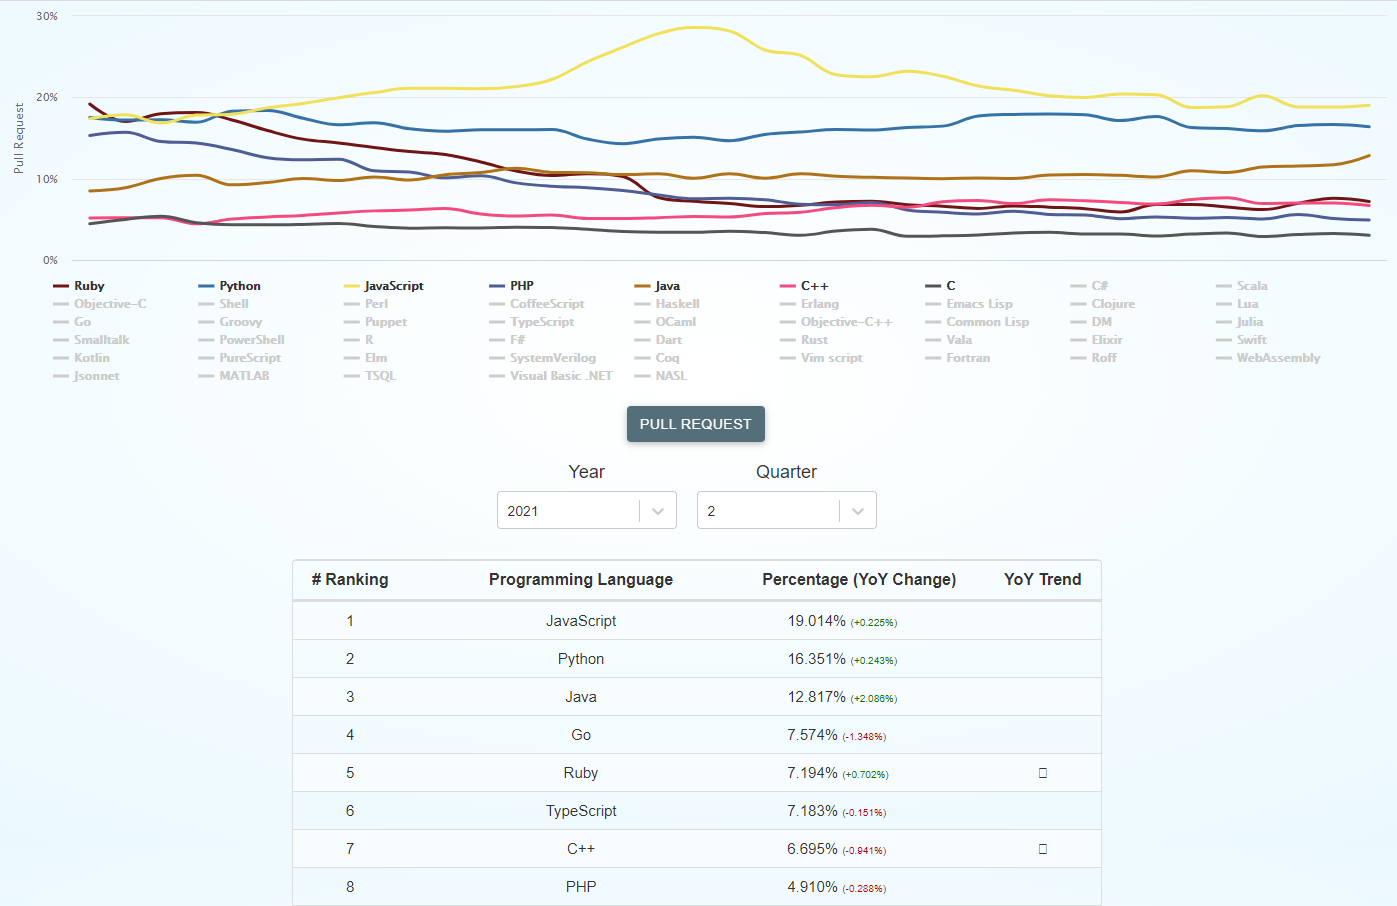
\includegraphics[width=16cm]{fig/github_languages.png}
	\caption{\it De meest populaire programmeertalen in de periode 2014-2021. Python is de tweede meest populaire taal, goed voor een zesde van alle (openbare) scripts ter wereld. \textit{Bron: GitHub}}
	\label{github-languages}
\end{figure*}

In deze periode komen de meest nuttige eigenschappen van Python aan de orde. Als je het begint te begrijpen, ga je de lol van programmeren vanzelf inzien. Maar zoals je eerst letters moet leren voordat je kunt lezen, moeten we beginnen met de wat taaiere kost waarvan het nut later duidelijk wordt: hoe maak en bewerk je een script, wat zijn datatypes, functies, variabelen, etc.

Een goede programmeur programmeert gestructureerd en begrijpelijk. Wat moet je hiervoor concreet doen?
\begin{itemize}
\item[-] Volg conventies: gebruik variabelen namen die aansluiten bij de inhoud van je programma: een lijst met temperatuurwaarden noem je niet \pythoninline{meuk}.
\item[-] Structureer je script: voeg scheidingen toe, definieer \textit{secties} met lege regels en kopjes (zoals je ook in normale tekst doet om hem leesbaar te houden).
\item[-] Voeg uitleg toe, vooral wanneer een stuk code moeilijk is. Hoe dit kan worden gedaan wordt later in deze reader behandeld.
\end{itemize}

Een goede stelregel is: \textit{Hoe moet ik een script schrijven zodat ik het zelf snel weer begrijp als ik het over een jaar open om te gebruiken}? In de beoordeling van deze periode is een deel van de punten gereserveerd voor de kwaliteit van de scripts om zo goed programmeren aan te moedigen.

\subsection{Python scripts schrijven en uitvoeren in Spyder}
We gebruiken op het Ichthus het programma Spyder om in te programmeren. De interface van Spyder wordt weergegeven in Figuur \ref{fig-spyder}. Deze bestaat standaard uit \'e\'en window met drie schermen: de Editor, Variable explorer en Console. Elk van deze heeft zijn eigen functie:
\begin{itemize}
\item[-] Het scherm links is de Editor. Hierin schrijf je de Python code, ook wel script genoemd, die een berekening of taak uitvoert. 
\item[-] De Explorer rechtsboven heeft vier tabbladen. Tab `Files' laat je scripts zien. In de Tab `Variable Explorer' wordt de waarde van de bestaande variabelen weergegeven nadat je een script hebt uitgevoerd. Alle figuren verschijnen in de Explorer onder de lab `Plots'. Tot slot geeft de `Help' tab je een mogelijkheid om snel de eigenschappen van een functie op te zoeken.
\item[-] De Console rechtsonder is het gedeelte waarin informatie over het runnen (of \textit{draaien}) van je script verschijnt. Ook de uitvoer (\textit{output}) komt hier terecht.
\end{itemize}

\begin{figure*}[h]
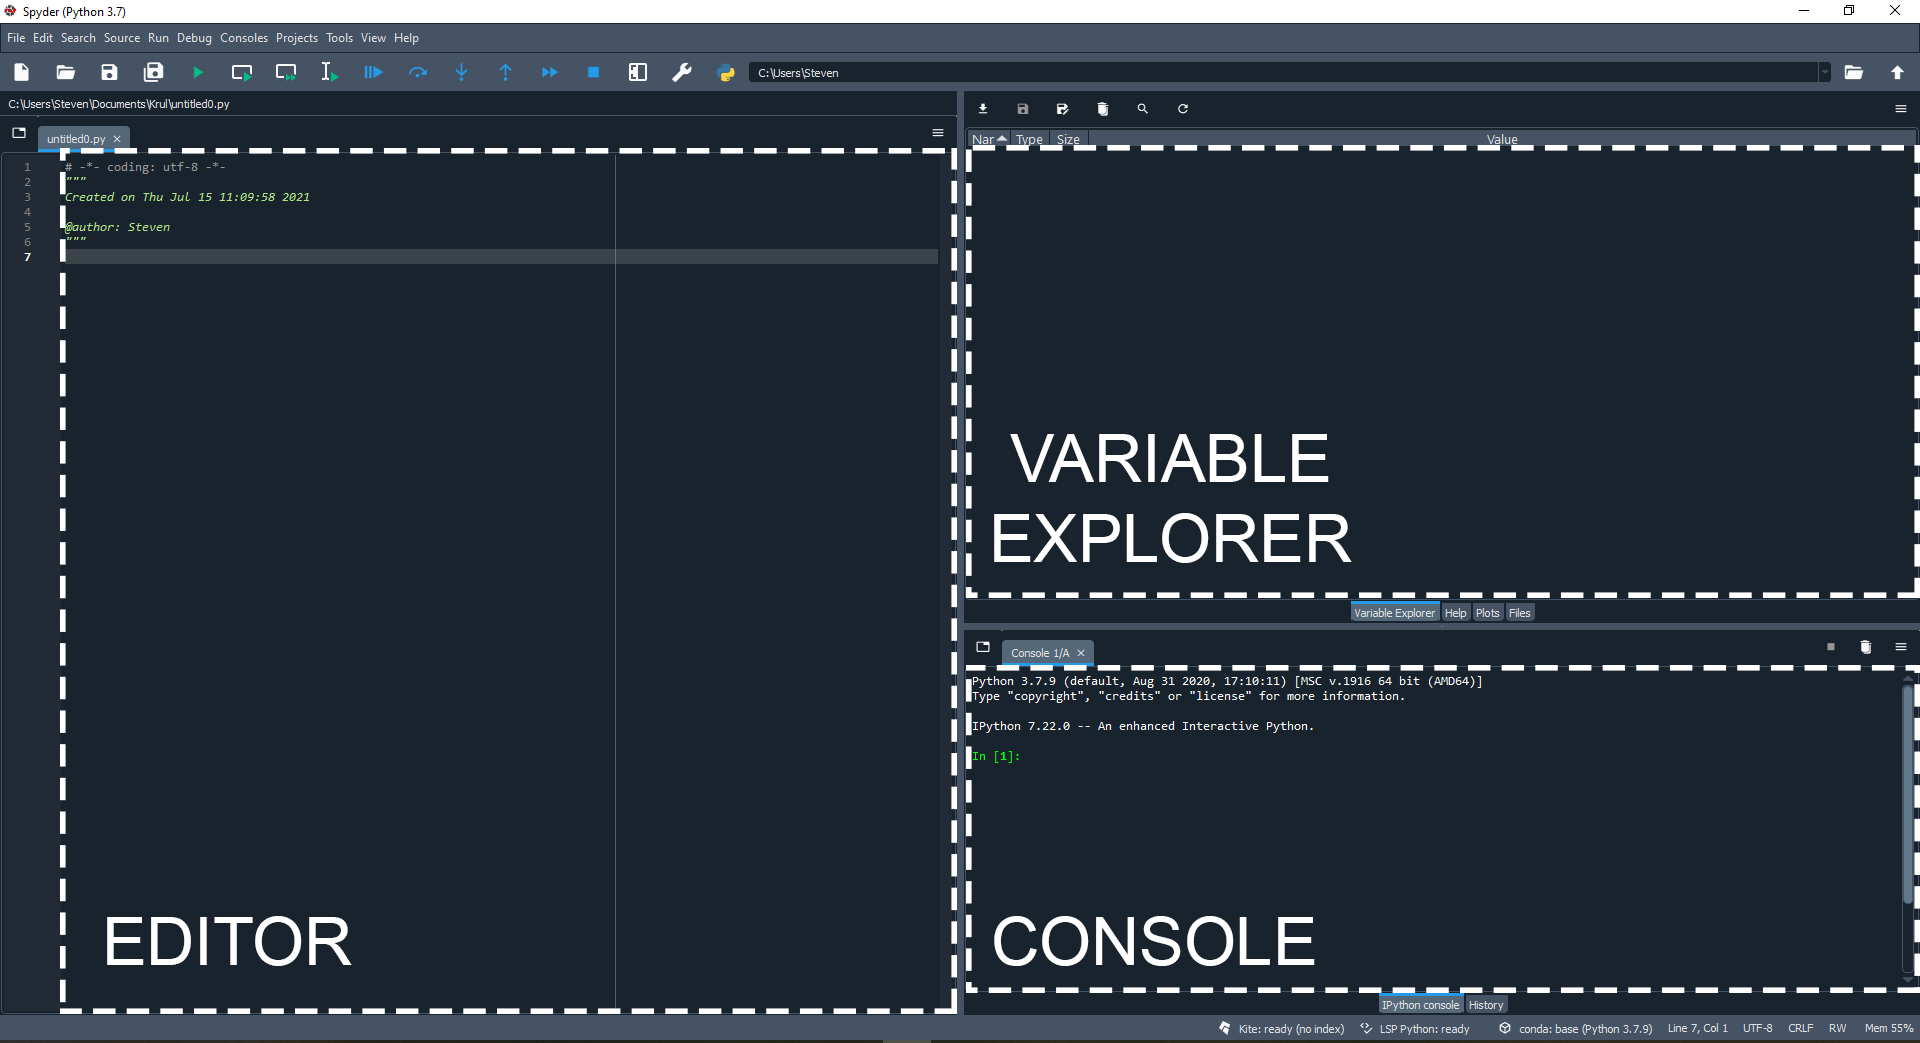
\includegraphics[width=16cm]{fig/spyder_screenshot.png}
\caption{\it De interface van Spyder direct na het opstarten van het programma.}
\label{fig-spyder}
\end{figure*}

Sla je bestanden met een duidelijke naam op in jouw GitHub map. Dit betekent dat de naam van de opgeslagen bestanden duidelijk maakt wat het script doet, of waar het onderdeel van is. Je kunt het beste alleen letters, cijfers en eventueel normale (-) of liggende (\_) streepjes (geen spaties!) te gebruiken. Een voorbeeld is de naam \verb,h1_1-helloworld.py,.

\subsubsection*{Oefenopdracht: Hello World} 
Typ de volgende regel tekst in de Editor: 
\begin{python}
print('Hello, world!')
\end{python}
Sla je bestand op met de naam \verb,h1_1-helloworld.py, en run het script.  Dat doe je door op de groene play-knop (of de F5-toets) in de balk bovenin te klikken.
Wat is de functie van het commando print? Kijk hiervoor in de console rechtsonderin.

Tijdens de periode zul je regelmatig (voorbeeld)scripts zien in deze bundel. Die kun je het beste openen via de hyperlink erboven. 
Sla deze als je ze nodig hebt op in je eigen map met bestanden en open deze vanuit Spyder op dezelfde manier waarop je dat in \textit{Word} zou doen\footnote{Kopie\"{e}r \textbf{niet} stukjes tekst uit de .pdf file die je nu leest naar het Editor window van Spyder, want dan krijg je vaak verminkte bestanden waaraan je onnodig veel tijd moet besteden om ze te repareren. Typ het over als het kort is, of klik op de hyperlink of ga naar ItsLearning om het hele bestand te vinden.}.

\subsection{Eenvoudige rekenkundige operaties}
Met Python kun je makkelijk rekenen. Hiervoor gebruik je normale tekens: optellen (\pythoninline{+}), aftrekken (\pythoninline{-}), vermenigvuldigen (\pythoninline{*}), delen (\pythoninline{/}) en (let op!) machtsverheffen (\pythoninline{**}). Een andere rekentruc die vaak voorkomt bij programmeren is de \textit{modulus} (\pythoninline{\%}). Dit is eigenlijk de 'rest'-berekening.

\begin{python}
1 + 1 # = 2
2 - 2 # = 0
3*3   # = 9
4/4   # = 1
5**5  # = 3125
5 % 2 # = 1
\end{python}

Tip: Het is onder Python programmeurs gebruikelijk om een spatie te typen voor en na een plus of min-teken, maar niet bij vermenigvuldigen, delen of machtsverheffen. Dit legt nadruk op de rekenregels. Bijvoorbeeld: 

\begin{python}
print(1 + 2 - 3*4**5) # wat komt hieruit?
\end{python}
\textbf{Vraag:} Wat is de betekenis van het \verb,#,-teken? Voer het script uit en je zult er dan wel achter komen. 

\textbf{Vraag:} Wat is het nut van \pythoninline{print()}?. Wat gebeurt er als je alleen de som berekent zonder \pythoninline{print()}?
\subsubsection*{Oefenopdracht: Python als rekenmachine} Bereken de hoogte $y$ van een softbal die vanaf de grond omhoog wordt geslagen met een beginsnelheid van $v_0 = 25 \, {\rm m/s}$ op $t = 2 \, {\rm s}$ aan de hand van de formule:
\begin{equation}
y = v_0 t - \frac{1}{2}g t^2
\label{eq-ball}
\end{equation}
De zwaartekracht $g = 9.81 \, {\rm m/s}^2$. Maak gebruik van het voorbeeld hiervoor.

\subsection{Variabelen}
\label{sec-vars}

\subsubsection{Implementatie}
Net als wiskunde `op papier' is het handig om van variabelen als letters gebruik te maken in plaats van de getallen gelijk in te vullen. Dit is ook zo bij programmeren en zorgt voor overzicht als je scripts langer en moeilijker worden.

Bij de vorige oefenopdracht moet je meerdere getallen aanpassen als je het tijdstip verandert. Maar veel handiger en sneller is het gebruik van {\it variabelen} in Python. Let op de volgorde waarin je de variabelen en de formule in je code opschrijft. Een script wordt (best logisch) van boven naar beneden uitgevoerd. Om berekeningen te kunnen doen met variabelen, moeten deze eerst gedefini\"eerd worden. Anders krijg je errors.

\begin{python}
a = 1
b = 2
c = 3
x = 1
y = a*x**2 + b*x + c
print(y)
\end{python}

Tip: Namen voor variabelen kun je zelf kiezen. De enige voorwaarden zijn dat de namen moeten beginnen met een letter, en geen spatie of wiskundig teken mogen bevatten.\footnote{Dus namen van variabelen (en later ook van functies) beginnen met een letter, bevatten alleen A-Z, a-z, 0-9 en \_ en zijn hoofdlettergevoelig.} Kies voor een variabele altijd een naam die past bij de betekenis ervan in jouw script. Noem een lijst van temperaturen bijvoorbeeld \pythoninline{temp} of \pythoninline{temperatuur}.

\subsubsection*{Oefenopdracht: Gebruik van variabelen} Bereken opnieuw de hoogte van de bal uit de vorige opdracht. Doe dit nu voor $t = 0,1,2,3, ... $ en geef een grove schatting hoe lang het duurt voordat de bal weer op de grond is. Nu maak je uiteraard gebruik van variabelen zoals hiervoor beschreven.

\subsubsection{Commentaar}
Vaak is het voor een buitenstaander een raadsel wat een variabele betekent als hij het script niet kent. 
Dit is \'e\'en van de redenen om in een script \textit{commentaar} toe te voegen. 
Het meest eenvoudig is het om hiervoor de hashtag te gebruiken, want alle tekst op een regel na \pythoninline{#} wordt genegeerd bij het runnen van een script. 

De oefenopdracht kan bijvoorbeeld op de volgende manier verduidelijkt worden:
\begin{python}
# hoogte softbal
v0 = 25	   # beginsnelheid in m/s
g  = 9.81  # zwaartekracht in m/s^2
t  = 2	   # tijdstip berekening
y = v0*t - 0.5*g*t**2 # formule voor de hoogte
print(y)
\end{python}
Als je in Spyder een nieuw Python script aanmaakt zie je direct nog een andere manier om commentaar te schrijven. Alle tekst tussen \verb,""", en de volgende \verb,""", is commentaar; deze manier van commentaar aangeven is handig voor grotere stukken tekst. 

\subsubsection{Datatypen}
In alle bovenstaande opdrachten zijn de variabelen hele getallen. Daarnaast kun je gebruik maken van stukken tekst, kommagetallen of \pythoninline{True/False}. Dat zijn allemaal {\it datatypen}. Hieronder de meest gebruikte, met hun offici\"ele naam:

\begin{description}
\item[\textbf{int}] Gehele getallen: \pythoninline{3  300  20}

In Python (en andere programmeertalen) is {\bf int} het datatype dat gebruikt wordt voor gehele getallen. Zie bovenstaand voorbeeld (\pythoninline{a = 1} etc). Je kunt ook een kommagetal gebruiken, maar let op: dit is niet hetzelfde als afronden op gehele getallen! \pythoninline{int(3.9) = 3} en niet een afgeronde 4.

\item[\textbf{float}] Getallen met decimalen: \pythoninline{2.3  4.62  100.00}

Het datatype voor decimale getallen is {\bf float}. Floats maak je door een getal met een decimale punt te maken, zoals: \pythoninline{a = 1.5}.

\item[\textbf{bool}] Logische waarde: \pythoninline{True} of \pythoninline{False}

Een {\bf boolean} type, dat we later in het hoofdstuk zullen tegenkomen, is een binair datatype dat twee waarden kan hebben: \pythoninline{True} of \pythoninline{False}. \pythoninline{True} is gelijk aan 1, en \pythoninline{False} is gelijk aan 0. \pythoninline{bool(1)} is dus gelijk aan \pythoninline{True}.

\item[\textbf{str}] Geordende reeks karakters (tekst): \pythoninline{'hello'  'Sam'  "2019"}

Een {\bf string} is het datatype voor tekst. Deze heb je ongemerkt gebruikt in de \pythoninline{'Hello world!'}, met \pythoninline{print()}. Om in Python een \pythoninline{string} te maken gebruik je aanhalingstekens. \pythoninline{a = 'tekst'} en \pythoninline{a = "tekst"} zijn allebei toegestaan.

\item[\textbf{list}] Geordende reeks objecten: \pythoninline{[10, "hello",200.3]}

Een \pythoninline{list} kan alle soorten datatypen bevatten, en die kun je ook los bekijken met behulp van een index. In hoofdstuk 2 komt hier meer van.

\end{description}

Je kunt het datatype van een variabele altijd bekijken in de Variable Explorer, als dat nodig is.

\subsection{Functies}
Je script kun je automatiseren door variabelen en de handelingen die je vaak herhaalt, in een \textit{functie} te zetten (een functie te defini\"eren).

\subsubsection{Eigengemaakte functies}
Een functie is een stukje tekst dat aan de hand van input \'e\'en of meerdere handelingen kan doen.

Functies worden vaak gebruikt om te voorkomen dat blokken code meerdere keren in een script herhaald worden. 
Hiermee zorg je ervoor dat, wanneer er een aanpassing gedaan moet worden, dit maar op \'e\'en plek hoeft te gebeuren. 
Ook blijft je script overzichtelijk, ook al maak je hem steeds langer of complexer. 

We gebruiken de formule $y = a x^2+b x + c$ om de werking van \textit{functies} uit te leggen. In het script hieronder zie je een voorbeeld van een functie die de waarde van de formule berekent en de uitkomst print op het scherm met behulp van de functie \pythoninline{print()}.

\begin{python}
def formule(a, b, c, x):
    y = a*x**2 + b*x + c   # bereken de formule
    return y               # geef de waarde terug

i = 1
j = 2
k = 3
z = 1
waarde = formule(i, j, k, z) # geef de variabelen mee op volgorde
print(waarde)
\end{python} 

Een Python functie begin je met het woord \pythoninline{def} ('definition'), gevolgd door de naam van de \textit{functie}. Daarna volgen tussen ronde haakjes de variabelen die door de functie moeten worden gebruikt als input. De regel wordt afgesloten met een dubbele punt om aan te geven dat wat er op de volgende regels staat de echte inhoud is. 

Daarna komt de code van de \textit{functie} zelf. Let op dat de regels code na het begin van de \pythoninline{def} niet helemaal links beginnen. Dit is belangrijk! De inspringing of \textit{indent} is onderdeel van de syntax van Python. Dit laat Python weten dat de tekst op die regel onderdeel is van de \textit{functie}. Spyder helpt je hierbij, want als je op Enter drukt komt deze indent er automatisch. Al moet je altijd even opletten. Wanneer de functie klaar is en je verder wilt gaan met de rest van een script, laat je de indent weg. Zo weet Python dat die regel niet bij de functie hoort.

Om een functie te gebruiken typ je de naam van de functie, met de waarden die je als input wilt gebruiken. De \textit{volgorde} van de variabelen vertelt welke waarde waar moet worden gebruikt. 
In bovenstaand voorbeeld krijgt parameter $a$ de waarde 1, want \pythoninline{i = 1}. Parameter $b$ krijgt de waarde 2, want \pythoninline{j = 2}.

Kijk na het overtypen (!) en runnen van bovenstaand script in de \textbf{Variable explorer} in Spyder. Hier kun je zien welke variabelen er bestaan, wat het type is en welke waarde ze hebben. De variabele \verb, waarde, heeft als het goed is de waarde 6. Dit getal moet ook afgedrukt zijn in de console door \verb,print,.

Een andere manier om waarden toe te kennen aan de variabelen binnen een functie is door de goede namen mee te geven. Dan maakt het niet meer uit in welke volgorde de variabelen een waarde krijgen toegekend. Bijvoorbeeld:

\begin{python}
# we geven de variabelen mee op een andere volgorde
waarde = formule(x=1, a=3, b=2, c=5) 
print('waarde = ', waarde)
\end{python}

Je moet in dit geval niet alleen weten dat de functie \verb,formule, vier argumenten verwacht, maar ook wat de naam van die argumenten binnen de functiedefinitie is. Samenvattend:
\begin{itemize}
\item Je geeft de argumenten op als een getal: de waarde van $a$ als eerste, etc.
\item Of: je geeft specifiek de waarden van $a$, $b$, $c$ en $x$ aan en dan mag je elke volgorde aanhouden.
\end{itemize}

\subsubsection*{Oefenopdracht: Controleren van bovenstaande functie}
Controleer dat \pythoninline{formule(3, 2, 5, 1)} en  \pythoninline{formule(x=1, a=3, b=2, c=5)} dezelfde waarde opleveren. Welke? En dat een \pythoninline{formule(1, 3, 2, 5)} een andere waarde oplevert. Controleer altijd je eigen functies met een simpele manier om fouten te voorkomen.

\subsubsection{Lokale vs. globale variabelen}
Het bovenstaande voorbeeld toont \'e\'en waarde op het scherm. Kijk je in het scherm van de \textbf{Variable explorer}, dan zie je dat alleen de variabelen \verb.i., \verb.j., \verb.k., \verb.z. en \verb.waarde. een waarde hebben, maar de \verb.a., \verb.b., \verb.c., \verb.x. en \verb.y. komen daarin niet voor.
De eerste variabelen zijn globaal (in het hele script) bekend en hebben de getoonde waarde. De andere variabelen zijn alleen bekend binnen de functie \verb.formule. en heten lokale variabelen. 

Waarden van lokale variabelen kun je hooguit weergeven door ze te printen binnen een functie, maar dat wordt al snel irritant als zo'n functie duizend keer wordt aangeroepen. 

Wat er binnen een functie gebeurt heeft normaal gesproken dus geen invloed op de rest van je script. Dit is een reden om onderdelen van een groter project op te bouwen uit functies.

Waarden van globale variabelen kun je wel gebruiken binnen een functie. Maar je kunt niet binnen een functie de waarde van een globale variabele veranderen.

Bij het gebruik van veel functies binnen een uitgebreid script is het al snel lastig om unieke korte namen voor variabelen binnen een functie te bedenken en kun je per ongeluk (of expres) meerdere keren dezelfde naam gebruiken. Dit zou er voor kunnen zorgen dat je script verkeerde resultaten oplevert. {\bf Noem je variabelen dus niet altijd zomaar \textit{a, b} en \textit{c}, maar geef ze een nuttigere naam waar mogelijk.}

\subsection{Loops}
%% While, if
Binnen Python bestaan manieren om functies of handelingen automatisch en/of heel vaak uit te voeren. We behandelen hier de constructies \pythoninline{while} en \pythoninline{if}.

\subsubsection{While}
Een zogenaamde \pythoninline{while} loop gebruik je om een bepaald stuk code te herhalen zolang er aan een voorwaarde voldaan wordt. Voor het voorbeeld van de omhoog geslagen bal dat we eerder gebruikt hebben kunnen we de hoogte van de bal berekenen voor de eerste $T$ seconden. Hoe zo'n loop kan worden ge\"implementeerd is te zien in onderstaand voorbeeld.

\begin{python}
v0 = 25   # beginsnelheid
g = 9.81  # zwaartekracht
t = 0.    # begintijd
dt = 0.25 # tijdstap

while t <= 5:
    y = v0*t - 0.5*g*t**2
    print(t, y)
    
    t = t + dt
\end{python}

Net als eerder defini\"eren we de benodigde variabelen $v_0$ en $g$. Daarnaast maken we een variabele aan voor de tijd $t$ en kiezen we de grootte van de tijdstappen $dt$ die we willen maken voor $t$. Zolang (\textit{while}) $t \leq 5$ wordt de hoogte $y$ berekend en worden $t$ en $y$ geprint.

Zolang $t\le5$ wordt aan de conditie voldaan en wordt de code in de functie van de \pythoninline{while} uitgevoerd. Om door te gaan naar de volgende tijdstap tellen we een stukje tijd $dt$ op bij $t$. 

Net als bij het gebruik van \pythoninline{def} moeten de regels code binnen de \pythoninline{while} \textit{loop} beginnen met een \textit{indent} om aan te geven dat die regels onderdeel zijn van deze \textit{loop}.

Een veelvoorkomende fout bij een \pythoninline{while} is dat de voorwaarde altijd \pythoninline{True} blijft, waardoor het script oneindig doorgaat. Dit gebeurt bijv. als je de regel \pythoninline{t = t + dt} vergeet of verkeerd invoert, of als je de regel wel goed overtypt maar de indent vergeet! Je kunt een script stoppen in Spyder door op de rode knop rechts boven in de Console te drukken.

\subsubsection{If}
Een tweede soort constructie is de zogenaamde \textit{if - else} constructie. Aan de hand van een voorwaarde (\textit{conditie}) wordt een bepaald deel code wel of niet uitgevoerd. Een variant hierop is de \textit{if - else if - else} constructie, waarbij er meer dan 2 mogelijkheden voorkomen. 

Let op: ook hier gebruik je \textit{indents}. In Python wordt \textit{else if} afgekort tot \pythoninline{elif}. 

\begin{python}
if gewicht < 40:            # 0 - 39.99999999 kg
    print("Ondergewicht!")
elif gewicht < 80:          # 40 - 79.99999999 kg
    print("Goed gewicht")
else:                       # 80 kg en meer
    print("Overgewicht!")
\end{python}


\subsubsection*{Oefenopdracht: Gebruik van \pythoninline{if} en/of \pythoninline{while}} 

\begin{itemize}
\item Schrijf een eenvoudig Python-script dat om input vraagt. Gebruik hiertoe: 
\begin{python}
invoer = input("Geef een positief getal: ")  # input heeft datatype string
getal = int(invoer)      # zet het om in een int, waar je mee kunt rekenen
\end{python}
Input moet je invoeren in de console. Als het opgegeven getal inderdaad positief is wordt de wortel\footnote{Weet je niet hoe je de wortel van een getal moet uitrekenen in Python? Zoek het dan op! Niet in deze reader, maar op internet.} van dat getal geprint en wordt er om nog een getal gevraagd. 
Is het opgegeven getal negatief, dan wordt de wortel niet uitgerekend. Je print dan de tekst \verb."Dombo: Positief svp!". en vervolgens vraagt het script (heel beleefd) weer om een positief getal. Maak dus gebruik van een loop! Pas als je de waarde 0 invoert stopt de loop en dus het script.
\end{itemize}

\subsubsection{Boolean expressions}
In de voorbeelden van loops hierboven hebben we voorwaarden gebruikt om delen van scripts wel of niet uit te voeren. De algemene term voor deze voorwaarde is \textit{Boolean expression}. De uitkomst van zo'n conditie heeft twee mogelijkheden, namelijk \pythoninline{True} of \pythoninline{False}. Vaak wordt zo'n voorwaarde ook wel een test genoemd.

\begin{python}
a == b	# test of a gelijk is aan b
a != b	# test of a niet gelijk is aan b
a > b	# test of a groter is dan b
a >= b	# test of a groter dan of gelijk is aan b
a < b	# test of a kleiner is dan b
a <= b	# test of a kleiner dan of gelijk is aan b
\end{python}

Daarnaast kunnen Boolean expressions ook worden gecombineerd door het gebruik van \pythoninline{and} waarbij de formule alleen  \pythoninline{True} zal opleveren als aan beide voorwaarden wordt voldaan; of \pythoninline{or} waarbij de formule \pythoninline{True} zal opleveren als aan minstens \'e\'en van de twee condities wordt voldaan (beide mag dus ook).

\begin{python}
a > b and c < d
a > b or c < d
\end{python}

\subsubsection*{Oefenopdracht: Testen van combinaties van Boolean expressions} 
\begin{itemize}
\item Neem het voorbeeld van de BMI over, een stukje terug. Voeg naast gewicht nog een voorwaarde toe: lengte. Je hebt alleen ondergewicht bij 40 kilo als je langer bent dan een bepaald aantal centimeter. Bedenk er zelf maar wat van, maar test je functie ook!
\end{itemize}

\subsubsection{For}
Als je een functie een exact aantal keer wilt uitvoeren kun je dit met een \pythoninline{while}- of \pythoninline{if}-loop doen waarin je een teller zet. Bijvoorbeeld:
\begin{python}
i=0
while i < 5:
    print(i)
    i=i+1
\end{python}
Een handigere manier om dit te doen is met een \pythoninline{for}-loop. Hierbij zit de `teller' automatisch ingebouwd: de loop wordt herhaald voor elk element in de voorwaarde. Elke \pythoninline{while}-loop is om te schrijven in een \pythoninline{for}-loop, maar soms \textit{voelt} de \'e\'en logischer, en is die ook makkelijker. Maar gebruik waar mogelijk een \pythoninline{for}-loop. Dit voorbeeld is toch best wat korter en simpeler:

\begin{python}
for k in range(5):
    print(k)
\end{python}

\subsubsection*{Oefenopdracht: for i in range()}
\begin{itemize}
	\item Voer het voorgaande stukje code uit. \\
	\textbf{Vraag:} welke getallen zitten er verborgen in \pythoninline{range(5)}? En wat als je er \pythoninline{range(10)} van maakt?
\end{itemize}

\subsection{Slotopdracht: Omrekenen van Fahrenheit naar Celsius}
{\it Voor alle opdrachten geldt dat je wordt aangemoedigd om op het internet te zoeken in de enorme hoeveelheid voorbeelden, tutorials, vragen en antwoorden over het gebruik van Python. Maak daar vooral gebruik van! Voor alle opdrachten geldt ook: maak je eigen script, en sla dat op met het nodige commentaar zodat je het later misschien kunt hergebruiken of je medestudenten er blij mee kunt maken.}

Schrijf een script waarin een reeks van verschillende temperaturen in Fahrenheit gebruikt wordt als invoer om te bepalen of het vriest of niet. Laat voor elke stap de temperatuur in Celsius zien samen met de conclusie of het wel of niet vriest. Test waarden van -10 t/m 100 Fahrenheit in stappen van 5 Fahrenheit. De conversie tussen Celsius en Fahrenheit is
\begin{equation}
C = \frac{5}{9}F - 32
\end{equation}

\clearpage
\renewcommand{\ditwc}{Modules (1): NumPy}
\section[Modules (1): NumPy]{\ditwc}
% Week 2
In dit hoofdstuk kijken we naar een essentieel onderdeel van het programmeren in Python: het gebruik van {\it modules}. Modules bevatten functionaliteit die niet in Python zelf zit maar apart toegevoegd moet worden. Oorspronkelijk kon je met Python niet veel meer dan stukken tekst bewerken. In dit hoofdstuk behandelen we \pythoninline{numpy}, dat het makkelijk maakt om met getallen en data te werken.

Het importeren van een module gebeurt (gewoonlijk op de eerste regel(s) van je script) met het commando \pythoninline{import}. Het is gebruikelijk om \pythoninline{numpy} af te korten tot \pythoninline{np}. Dat ziet er in de praktijk zo uit: 
\begin{python}
import numpy as np
\end{python}
Vanaf dit punt wordt naar \pythoninline{numpy} verwezen als \pythoninline{np}. Om functies uit een module te gebruiken wordt de afkorting van de module als voorvoegsel gebruikt, gevolgd door een punt, en dan het commando(= de naam van de functie) uit de module.\\
Bijvoorbeeld: \pythoninline{np.sin(X) # berekent de sinus van X}.

\subsection{Arrays maken}
Een {\it array} (Nederlands: reeks) is een verzameling van getallen. In Python kun je die maken als een lijst (zie hoofdstuk 1.3.3), maar een lijst is in de praktijk heel erg onhandig. In plaats van een lijst gebruiken we veel liever een numpy array. Hier kan maar \'e\'en datatype tegelijkertijd in voorkomen: \pythoninline{ints} of \pythoninline{floats}.

De duidelijkste manier om een array te maken is met de functie \pythoninline{np.array()}. Als je de getallen van de dobbelsteen in een array wilt zetten, doe je dat bijvoorbeeld zo:
\begin{python}
getallen_array = np.array([1,2,3,4,5,6]) 
# let op de extra blokhaken [] tussen de ronde haken ()
\end{python}

Handmatig alle getallen invullen is iets waar je als programmeur niet op zit te wachten. Als het ook maar een klein beetje kan, doen we dat het liefst automatisch. In het codeblok hieronder staan een aantal manieren om automatisch arrays aan te maken.

\pythonexternal{code-inc/w2/np_vb1.py}

Merk op dat \pythoninline{np.arange()} het eindgetal (\pythoninline{5.}) niet meeneemt, \pythoninline{np.linspace()} doet dit wel, dus \pythoninline{grid1} en \pythoninline{grid2} zijn verschillend. 

\subsubsection*{Oefenopdracht: Maken en bewerken van numpy arrays}
\begin{itemize}
	\item[a)] Schrijf een script waarmee een array wordt gemaakt met daarin de getallen 1.5 tot en met en 3.0 met stappen van 0.3. Doe dit met zowel \pythoninline{np.arange} als \pythoninline{np.linspace}. Controleer je resultaten met \pythoninline{print()}.
	
	{\bf Tip}: Begin met \pythoninline{xmin = 1.5}, \pythoninline{xmax = 3.0} en \pythoninline{dx = 0.3}. Werk daarna alleen met deze variabelen, of andere hulpvariabelen die volgen uit deze 3 variablen.
	
\end{itemize}

\subsection{Rekenen met arrays}
Rekenen met arrays is super makkelijk. Wanneer twee arrays dezelfde vorm (evenveel getallen) hebben, kun je ze getal voor getal optellen door \pythoninline{+} te gebruiken. Wanneer deze niet dezelfde vorm hebben krijg je een foutmelding. Alle wiskundige formules (\pythoninline{+,-,/,*,**}) werken op deze manier.

Neem het volgende voorbeeld maar over en zie wat er gebeurt:
\begin{python}
a = np.array([1,2,3,4,5])
b = np.array([6,7,8,9,10])
c = a + b
print("c: ", c)
d = a * b
print("d: ", d)
\end{python}

\subsubsection*{Oefenopdracht: Maken en bewerken van numpy arrays}
\begin{itemize}
	\item[b)] Schrijf een script dat een array maakt met de gehele getallen tot en met 10, beginnend bij 1. Natuurlijk geef je dat array een naam. Print en controleer de resultaten. Valt je iets op?\footnote{Als er iets niet klopt, geef het aan bij de docent! Die legt het wel uit :)}
\end{itemize}

\subsection{Indexing en slicing}
Soms is het fijn om delen van een array een aparte naam te geven. Of je wilt een specifiek getal uit een getallenreeks halen. In het codeblok hieronder is te zien hoe je een enkel element uit een array kunt selecteren {(\it indexing} of een groter deel van de array {\it slicing}). Door gebruik te maken van {\it slicing} bekijk je de {\it oorspronkelijke} data van de array. Wijzig je de data in de slice, dan wijzig je dus ook de data in het oorspronkelijke array!

\pythonexternal{code-inc/w2/np_vb2.py}

Let dus goed op het verschil tussen de laatste twee handelingen: \pythoninline{kopie_arr} is een kopie van de waarden, terwijl \pythoninline{same_arr} alleen een andere naam is voor \pythoninline{test_array}!

\subsubsection*{Oefenopdracht: Maken en bewerken van numpy arrays}
\begin{itemize}
	\item[c)] Vraag: wat is de waarde van \pythoninline{test_array[1]}? Let goed op!
	
	Een computer begint bij nul te tellen. Dat betekent dat het eerste getal, wat bij ons altijd plek 1 krijgt (bijvoorbeeld vers 1 van een hoofdstuk in de Bijbel), voor de computer op plek 0 staat. En het vijfde getal in een reeks staat voor de computer op plek 4.
	
	\item[d)] Neem de laatste regel (en het bijbehorende \pythoninline{test_array}) over van bovenstaand voorbeeld. Print eerst de laatste getallen van beide arrays (\pythoninline{test_array} en \pythoninline{same_arr}). Voeg vervolgens daaronder deze regel toe: \pythoninline{test_array *= 10}. Daarmee vermenigvuldig je het \pythoninline{test_array} met 10. Print weer beide getallen. Zet daaronder deze regel: \pythoninline{test_array = test_array / 5}, en print weer beide getallen. Wat is het verschil? Vraag het als je het niet snapt!
\end{itemize}

\subsection{Allerlei functies}
Numpy arrays hebben een aantal ingebouwde functies, om bijvoorbeeld het gemiddelde of de som uit te rekenen. Ook de lengte of de vorm en datatype worden verkregen door \pythoninline{.functie} aan de naam van zo'n array vast te plakken.

\pythonexternal{code-inc/w2/np_vb3.py}

Let op de laatste regel: dit is eigenlijk iets meer werk, maar over het algemeen veel veiliger! Als je bijvoorbeeld de mediaan van een array uit wilt rekenen, kun je {\it niet} gebruik maken van \pythoninline{test_array.median()}, maar moet je de andere methode gebruiken: \pythoninline{np.median(test_array)}.

\subsection{Maskers}
In sommige gevallen wil je een lijst getallen ook filteren. Je bent bijvoorbeeld geïnteresseerd in alle leeftijden boven de 18 jaar, of alle leerlingen in de bovenbouw. Dit kan aan de hand van een {\it masker}. De werking van zo'n masker wordt uitgelegd aan de hand van het onderstaande voorbeeld
\footnote{In de .pdf zie je dat diverse Python woorden blauw gekleurd zijn; ook als er in een stukje tekst toevallig een Python woord staat, zoals in masker. Een klein foutje waar ik helaas niet veel aan kan doen.}.
Een masker maak je door een voorwaarde op te geven bij een variabele. Alle plekken in de array die voldoen aan die voorwaarde, geven de waarde \pythoninline{True}, alle anderen geven \pythoninline{False}. Een masker pas je vervolgens toe met de blokhaken \pythoninline{[ ]}.

\pythonexternal{code-inc/w2/np_vb4.py}

\subsubsection*{Oefenopdracht: Maken en bewerken van numpy arrays}
\begin{itemize}
	\item[e)] Bereken het gemiddelde van het $k^k$-array van oefenopgave b).
	\item[f)] Selecteer met behulp van een masker alle oneven getallen uit \pythoninline{test_array} van bovenstaand voorbeeld.
\end{itemize}

\iffalse
\subsection{Reshaping}
Tot nu toe hebben we alleen met \'e\'endimensionale arrays gewerkt - een lijst van alleen getallen achter elkaar. Je kunt echter ook meerdimensionale arrays maken: 2D, 3D of in theorie zelfs veel meer dimensies. Wanneer je werkt met meerdimensionale lijsten kan het handig zijn om de vorm van de array aan te passen. De meest gebruikte bewerking is \pythoninline{np.ravel()}, die elke meerdimensionale array verandert in een \'e\'endimensionale array door alle elementen achter elkaar te zetten.

Het commando \pythoninline{np.reshape()} maakt juist van een \'e\'endimensionaal array een meerdimensionale array met afmetingen afhankelijk van de opgegeven parameters.\footnote{Deze commando's werken alleen op \pythoninline{numpy array}'s, niet op objecten van bijvoorbeeld type \pythoninline{list}.}

\pythonexternal{code-inc/w2/ravel_vb1.py}

\subsubsection*{Oefenopdracht: sorteren en reshapen}
\begin{itemize}
	\item[f)] Laat \pythoninline{y = np.arange(30); np.random.shuffle(y)}. Wat is de werking van \pythoninline{np.random.shuffle()}? Schrijf een script dat \pythoninline{y} verandert in een gesorteerd array van 2 bij 15, waar de bovenste rij de 15 oneven getallen gesorteerd bevat en de onderste rij de 15 even getallen. Gebruik \pythoninline{np.sort()} om de lijst weer te sorteren, en maak slim gebruik van \pythoninline{np.reshape()} en de commando's uit bovenstaand voorbeeld om de even en oneven getallen te scheiden.
\end{itemize}

\subsection{Samenvoegen}
E\'en of meerdere elementen toevoegen aan het einde van een \'e\'endimensionaal array gaat het beste met de functie \pythoninline{np.append()}. Zie het voorbeeld:

\begin{python}
array1 = np.array([1,2,3,4,5])	   # array ziet eruit als [ 1 2 3 4 5]
array2 = np.append(array1, 6)	   # array ziet eruit als [ 1 2 3 4 5 6]
array3 = np.append(array2, [7, 8]) # array ziet eruit als [ 1 2 3 4 5 6 7 8]
\end{python}

Het achter elkaar plakken van twee numpy arrays kan met de functie \pythoninline{np.concatenate()}. Deze functie is ook goed bruikbaar voor meerdimensionale arrays. Standaard gaat dit langs de x-as, maar de as waarlangs het samengevoegd wordt kun je aanpassen met \pythoninline{axis=..}. De x-as is as 0, de y-as is as 1, en als een array driedimensionaal is, is de derde as de z-as, met waarde 2.

\pythonexternal{code-inc/w2/conc_vb1.py}

Neem dit script over en kijk goed naar de dimensies. Print de arrays, of bekijk ze in de Variable explorer. Verander een paar getallen en zoek uit wat wel en niet werkt!
\fi

\subsection{For-loops}
De structuur van een \pythoninline{for}-loop is altijd:
\begin{python}
for element in data:
	voer_functie_uit_voor_element
\end{python}
Het Python key-woord \pythoninline{in} komt hierin dus altijd voor evenals de \pythoninline{:} aan het eind. Cruciaal is dat \pythoninline{data} elementen bevat. E\'en zo'n element kun je noemen zoals je wilt, dus kies een nuttige naam. Kun je geen nuttige naam bedenken, dan is \pythoninline{i} eigenlijk de standaard. Vervolgens voer je berekeningen uit voor elk element. De volgende voorbeeld-code maakt dat duidelijk.

\pythonexternal{code-inc/w2/for_vb1.py}

\subsection{Slotopdracht: Voortschrijdend gemiddelde}
Tijdens de corona pandemie hebben we eindeloos veel grafiekjes gezien van het aantal besmettingen per dag. In het weekend is dat altijd lager, en door de weeks juist weer hoger. Het is daarom nuttiger om naar het gemiddelde van de afgelopen zeven dagen te kijken: dan compenseer je de uitschieters een beetje. Dit gemiddelde noemen we het {\it voortschrijdend gemiddelde}: voor elke dag bereken je het gemiddelde van de zeven dagen daarvoor. Je kunt over de eerste 7 dagen geen voortschrijdend gemiddelde berekenen: er zijn immers nog geen volledige zeven dagen geweest.

In deze slotopdracht maak je zelf een voortschrijdend gemiddelde.

\begin{itemize}
	\item Maak een array van 50 random getallen tussen de 0 en 1 (zoek hiervoor in het hoofdstuk).
	\item Maak een variabele genaamd \pythoninline{periode}, met de waarde 7. Dit is het aantal dagen waarover we het gemiddelde gaan berekenen.
	\item Start vervolgens een \pythoninline{for}-loop toe. Deze gaat lopen van de dag n\'a de periode, tot en met de laatste waarde van je array.
	\item Bereken per element in de \pythoninline{for}-loop het gemiddelde van de afgelopen 'periode' dagen. Voeg dit gemiddelde toe aan een array met de voortschrijdende gemiddeldes.
	\item Print na afloop van de loop de array met voortschrijdende gemiddeldes. Wat valt je op als je de periode verhoogt (naar bijvoorbeeld 20)?
\end{itemize}

\clearpage
\renewcommand{\ditwc}{Modules(2): MATPlotLib}
\section{Modules (2): MATPlotLib}
%Week 3
In dit deel bekijken we hoe we data kunnen visualiseren: zichtbaar maken in grafieken. We gebruiken hiervoor het \pythoninline{pyplot} onderdeel uit het pakket \pythoninline{matplotlib} (MATLab Plotting Library). Het importeren werkt vergelijkbaar als bij \pythoninline{numpy}:
\begin{python}
import matplotlib.pyplot as plt
\end{python}

\subsection{Grafiek maken}
Hieronder een voorbeeld om een sinus in beeld te brengen.
\pythonexternal{code-inc/w3/plt_vb1.py}

\subsubsection*{Oefenopdracht}
\begin{itemize}
	\item[a)] Imiteer het bovenstaande voorbeeld. Verander het aantal elementen in \pythoninline{x}. Wat gebeurt er als het aantal elementen in de lijst klein is? (bijvoorbeeld 10)

	\item[b)] Voeg een cosinus toe door een \pythoninline{y2} te defini\"eren en een extra \pythoninline{plt.plot()} toe te voegen. 

	\item[c)] Maak een extra plaatje (door in hetzelfde script een nieuwe \pythoninline{plt.figure()} toe te voegen) waar \pythoninline{y} en \pythoninline{y2} tegen elkaar uitgezet worden. In plaats van \textit{x} en \textit{y} in \pythoninline{plt.plot(x,y)} moet je dus wat anders invoeren.
\end{itemize}

\subsection{Lijnen opmaken}
Wanneer twee grafieken in \'e\'en figuur getekend worden, zoals hiervoor, geeft \pythoninline{plt} automatisch de tweede lijn een andere kleur. Om zelf kleur en stijl in te stellen is het mogelijk om een aantal commando's toe te voegen aan \pythoninline{plt.plot()}.

\pythonexternal{code-inc/w3/plt_vb2.py}

\subsubsection*{Oefenopdracht (vervolg)}
\begin{itemize}
	\item[d)] Pas het script van b) aan zodat de sinus als rode lijn en cosinus als magenta punten geplot worden.

	\item[e)] Bij het aanroepen van de \pythoninline{plt.plot()}, voeg de optie \pythoninline{label = "Label van grafiek"} toe binnen de haakjes van \pythoninline{plt.plot()}. Label de sinus ``Sinus'' en de cosinus ``Cosinus''. Gebruik vervolgens het commando \pythoninline{plt.legend()} onder de plot-functies om een legenda weer te geven.
	
	\item[f)] De waarden op een bepaalde plek op de lijn zijn niet altijd zo makkelijk af te lezen bovenin of rechts in de figuur. Hier komt \pythoninline{plt.grid()} goed van pas. Hoe zit je figuur er uit als je dit toevoegt?
\end{itemize}

\subsection{Assen opmaken}
Een grafiek zonder tekst is (bijna) helemaal nutteloos. Zien we de windsnelheid, of de temperatuur, en dan in graden Celsius of Farenheit? En gaat het over de uren op een dag of over de maandnummers? Cruciale info, die aanwezig moet zijn in een grafiek. Uiteraard helpt \pythoninline{pyplot} ons hier ook weer een handje met een aantal nuttige functies. Zie onderstaand voorbeeld:

\pythonexternal{code-inc/w3/plt_vb5.py}

\subsubsection*{Oefenopdracht (vervolg)}
\begin{itemize}
	\item[g)] De lijn in het plaatje van het voorbeeld toont gaten aan de linker- en rechterkant. Pas met \pythoninline{plt.xlim(x_min,x_max)}  het bereik van de $x$-as aan. Maak het bereik van de $x$-as $1981$ tot $2021$. Je kunt het bereik op de $y$-as ook op dezelfde manier aanpassen. Zet het bereik van de $y$-as van $30$ tot en met $50$.
	
	\item[h)] In het plaatje van c) (wat een cirkel zou moeten tonen) is de verhouding van $x$- en $y$-as niet ingesteld. Zet de aspectratio (verhouding) op 1 met \pythoninline{plt.axes().set_aspect('equal')}. In plaats van \pythoninline{'equal'} kun je ook \pythoninline{1} invullen (verhouding 1:1).
	
	\item[i)] Maak de volgende plot: kies $t$ van $0$ tot $2\pi$. Laat $x = 16 \sin^3(t)$ en $y = 13 \cos(t) - 5 \cos(2t) - 2 \cos(3t) - \cos(4t)$. Zorg voor een goede verhouding tussen de assen.
\end{itemize}

\subsection{Meer grafieken in \'e\'en figuur}
Soms is het fijn om twee plots boven elkaar of naast elkaar te laten zien, eventueel zodat ze de x- of y-as delen voor het overzicht (ze hebben dan hetzelfde bereik). Om meerdere plots tegelijk te laten zien kan de functie \pythoninline{plt.subplots()} gebruikt worden. \pythoninline{plt.subplots()} maakt van elk figuur (subplot) een apart object, waarop je met \pythoninline{axN.plot()} en gelijke functies figuren kunt plotten. Hier is de naam \pythoninline{ax} niet verplicht, maar heel veel voorbeelden op internet werken met deze naam, dus doen we dat hier ook.

\pythonexternal{code-inc/w3/plt_vb3.py}

Een tweede voorbeeld waar plotjes in een 2-bij-2 vorm worden getoond.

\pythonexternal{code-inc/w3/plt_vb4.py}

Merk op dat gebruik wordt gemaakt van een 2-bij-2 array om de informatie voor de individuele plots op te slaan. De eerste index (het eerste getal) tussen de blokhaken staat daarbij voor de x-as, het tweede getal voor de y-as. Let op: Python begint linksbovenin met \pythoninline{[0,0]}, en heeft \pythoninline{[0,1]} linksonderin staan. De y-as loopt dus naar beneden in plaats van naar boven. De x-as `klopt' wel.

\subsubsection*{Oefenopdracht (vervolg)}
\begin{itemize}
	\item[j)] Maak een figuur met twee subplots: plot in de ene een sinus, en in de andere een cosinus. Kies de x-as tussen 0 en $2\pi$ met behulp van \pythoninline{axN.xlim(x_min, x_max)}. Voeg in allebei de plots de legenda toe. HINT: vervang \pythoninline{plt} nu door \pythoninline{ax1} en \pythoninline{ax2}.
\end{itemize}

\subsection{Slotopdracht: Heel veel plotjes}
Maak een figuur van 2-bij-2 plots waarin net als in het voorbeeld met de drie plotjes de $x$-markering weggelaten is voor figuren die niet onderaan staan. Laat ook de $y$-markering weg voor figuren die niet helemaal links staan. 
De plots moeten er als volgt uit zien: voor elke plot is het bereik voor $x$ gelijk aan $[0,1]$. In elke plot moet $x^\alpha$ komen staan. In linksboven voor $\alpha = 0.125,0.25,0.5,1$, in rechtsboven $\alpha = 1,1.5,2$, in linksonder $\alpha = 1,2,3,4$ en rechtsonder $\alpha = 0.1,1,10$. Je kunt dit met de hand, regel voor regel doen, maar de uitdaging van deze opdracht zit hem vooral in het zo compact en efficiënt mogelijk maken van je script. Voeg achteraf ook labels en legenda toe en maak de figuur met behulp van de geleerde dingen in dit hoofdstuk zo netjes mogelijk.


\clearpage
\renewcommand{\ditwc}{Importeren en exporteren}
\section[Importeren en exporteren]{\ditwc}
% Week 4
Voor het verwerken van data ben je eigenlijk altijd afhankelijk van losse bestanden die alle gegevens bevatten. Niemand gaat voor de lol duizenden getalletjes met de hand invoeren: dan kun je net zo goed Excel gebruiken. Ook wil je graag je gemaakte figuren en resultaten opslaan om ergens in te voegen: anders kun je net zo goed maar wat met de hand tekenen of berekenen. Maar daar doen we het niet voor: we gaan handelingen automatiseren door bestanden te \textit{importeren}, en vervolgens resultaten te \textit{exporteren}. Dat gaan we dit hoofdstuk behandelen.

\subsection{Afbeeldingen exporteren}
In het vorige hoofdstuk heb je al geleerd om plaatjes te maken. Figuren staan normaal gesproken alleen in Spyder, en kunnen niet direct gebruikt worden in een verslag, artikel of rapport. Daarvoor moet je de afbeelding eerst opslaan. Hiervoor kan je gebruik maken van \pythoninline{plt.savefig()}.

De belangrijkste opties die je aan deze functie kunt meegegeven zijn de naam van de afbeelding en de resolutie. De standaard locatie waar de afbeelding wordt opgeslagen is de map waar het script is opgeslagen. 

Als bestandstype kan er worden gekozen voor \verb.jpg., \verb.png. en  \verb.pdf.. 
De resolutie van deze afbeeldingen wordt gespecificeerd in \textit{dots-per-inch}  (\verb,dpi,).
Afbeeldingen van het type .jpg en .png kun je niet zo ver inzoomen, omdat op een gegeven moment de pixels zichtbaar worden. 
Afbeeldingen van het type .pdf zijn opgebouwd uit formules zoals punten, lijnen en/of krommen. Ook gewone letters hebben zo'n structuur. Daardoor kun je zo ver inzoomen als je zou willen zonder dat het onscherp wordt.

Met behulp van \pythoninline{plt.figure(figsize=[breedte, lengte])} kun je instellen hoe groot je plaatje is, en welke verhoudingen hij heeft. Hoe groter de breedte en lengte, hoe groter het bestand.

\pythonexternal{code-inc/w4/export_vb1.py}

\subsubsection*{Oefenopdracht} 
\begin{itemize}
\item Open het onderstaande voorbeeld-script \verb,export_vb2.py,. Je kunt met dit voorbeeld ook makkelijk meerdere figuren in \'e\'en script aanmaken.
\item Verander het script zodat het een aantal plaatjes van alleen de sinus-functie maakt. 
Om niet steeds hetzelfde plaatje te krijgen varieer je met de volgende instellingen:

\begin{enumerate}
\item De extensie van het weggeschreven bestand. Kies: \verb,png, of \verb,pdf,. Hierin is al voorzien in het voorbeeld door tweemaal een \verb,plt.savefig, te doen.
\item De grootte van het plaatje. Kies bijv. \verb=[2,1]= of \verb=[20,10]=.
\item Het aantal dots-per-inch. Kies bijv. 300 of 1200. (Zie het vorige voorbeeld!)
\end{enumerate}

\item Open de plaatjes en kijk naar de kwaliteit. Gebruik de zoom-functie! Kijk ook naar de bestandsgrootte (in kilobytes) van de aangemaakte bestanden. Trek je conclusie!

\pythonexternal{code-inc/w4/export_vb2.py}

\end{itemize}

\iffalse
\subsection{For-loops}
\label{Ch_forloop}

Eerder zijn we uitgebreid ingegaan op een speciaal soort lijsten, \pythoninline{numpy}-arrays, omdat deze heel erg geschikt zijn voor data-analyse. 
Het rekenen met \pythoninline{numpy}-arrays is heel erg efficiënt (er is weinig code nodig) en snel (er is weinig computertijd nodig). Je kunt over het algemeen veel beter een array gebruiken dan een Python list. Run het volgende voorbeeld maar eens:  

\pythonexternal{code-inc/w4/forloop_vb1.py}

Omdat een Python lijst uit allemaal verschillende datatypen kan bestaan, werkt dat in een \pythoninline{for}-loop totaal niet goed. Daar heb je het liefst dat alles op dezelfde manier werkt, zodat je op elk element dezelfde berekening of handeling kunt doen.
Zo kun je de gehele lijst, van begin tot eind, op dezelfde manier bewerken.

\subsubsection*{Oefenopdracht: Spelen met lijsten en printen binnen for-loop} 

\begin{itemize}
\item Maak een \pythoninline{numpy} lijst $l_1$ met 100 elementen: de gehele getallen 0 tot en met 99.
Vermenigvuldig elk getal in die lijst met 100; noem deze lijst $l_2$.
\item Maak een nieuwe lijst $ l_3 = l_2 - l_1^2$.
Sorteer de elementen in $l_3$. 
\item Zorg ervoor dat de 9 grootste elementen van $l_3$ in aflopende volgorde in een lijst $l_4$ terechtkomen (die dus 9 elementen bevat).
\item Maak nu een nieuwe lijst $l_5$ die deze 9 waarden bevat, alleen nu geordend als een 3 bij 3 array. Dit is dus een twee-dimensionaal array. Het eerste element bevat de 3 grootste getallen, etc.
 \begin{itemize}
  \item Druk nu de gehele lijst $l_5$ met \'e\'en print af. 
  \item Druk ook elk element van de lijst $l_5$ af in een \pythoninline{for}-loop over alle elementen van $l_5$. Let er hierbij op dat $l_5$ stiekem maar 3 elementen heeft (met elk weer 3 elementen)! 
 \end{itemize}
 Noteer de verschillen in de afgedrukte output. 
\end{itemize}
\fi

\subsection{Formatteren van tekst}
\label{sec:format}

In het begin hebben we losse waarden op het beeldscherm getoond: vaak dus \'e\'en getal per regel, maar er kunnen ook meerdere berekende waarden in een keer op het scherm worden getoond met \'e\'en \pythoninline{print} statement. Dit kan door meerdere variabelen op te geven gescheiden door komma's.

\begin{python}
a = 1
b = 2
c = 3
print('a =', a, 'b=', b, 'c=', c)
\end{python}

Het kan handig zijn tekst toe te voegen, zodat berekende waarden meer voor zichzelf spreken, zoals in onderstaand voorbeeld.

\begin{python}
print('Na ', t, 'seconden, is de bal', y, 'meter hoog.')
\end{python}

Een andere manier om tekst te tonen op je beeldscherm kan met behulp van \pythoninline{format}. Je hoeft dan veel minder komma's en quotes te gebruiken en hebt er meer controle over. Het is dan niet langer nodig verschillende stukken te scheiden met komma's, maar je gebruikt een enkele \pythoninline{string}. Hierin geef je met accolades (\pythoninline{\{\}}) aan waar de waarden van variabelen kunnen worden ingevuld en sluit je af met de functie format, waarin je de namen van de variabelen aangeeft.

In de accolades kun je met een code aangeven hoe je tekst er uit komt te zien. Deze {\it codes} beginnen met een dubbele punt gevolgd door een aantal letters. Zie tabel \ref{tab:format} voor een aantal mogelijkheden.

\begin{table}[ht]
\caption{Codes voor het weergeven van gegevens.}
\label{tab:format}
\begin{center}
\begin{tabular}{ r l l }
\hline
:d    & integer & \pythoninline{500}\\
:.xf  & decimale notatie met $x$ decimalen & \pythoninline{500.00} ($x=2$)\\
:.xe  & wetenschap. notatie met $x$ decimalen & \pythoninline{5.0e+02} ($x=1$)\\
:s    & string & \pythoninline{'5'}\\
\hline
\end{tabular}
\end{center}
\label{default}
\end{table}%

\subsubsection*{Oefenopdracht: Oefenen met het precies formatteren van tekst}
\begin{itemize}
\item
Verander de manier waarop de getallen $t$ en $y$ worden geformatteerd. 
Hoeveel correcte decimalen van \pythoninline{np.pi} kun je zo op je scherm te zien krijgen? 
(Antwoord: 15). 
Probeer behalve het aantal decimalen te vari\"eren ook te spelen met het type door $t$ en $y$ af te drukken als string of integer! 
Let op wat er dan gebeurt. Je kunt gebruik maken van onderstaand voorbeeld:
\begin{python}
t = np.pi
y = 22/7
print('Na {} seconden is de bal {} meter hoog'.format(t,y))
print('Na {:.2f} seconden is de bal {:.2f} meter hoog'.format(t,y))
\end{python}
\end{itemize}

\iffalse
\subsection{Exporteren}

Naast afbeeldingen is het noodzakelijk om de achterliggende gegevens te bewaren voor later gebruik. Hiervoor zijn talloze types bestanden beschikbaar, elk toegespitst op een bepaald soort gegevens. Hoewel er erg geavanceerde bestandstypes bestaan die weinig ruimte in beslag nemen of erg snel werken met bepaalde programma's, zullen we ons in deze cursus beperken tot tekstbestanden (.txt of .csv). Deze bestanden zijn leesbaar voor de mens, wat uiteraard fijn is.

Structuur aanbrengen in een bestand is noodzakelijk. Dit begint bij het ordenen van je data. Daarnaast is het ook belangrijk om extra informatie (ook wel \textit{metadata}) aan het bestand toe te voegen. Denk aan namen van variabelen, maar ook meetomstandigheden, de datum en andere informatie die een gebruiker van het bestand nodig heeft om de gegevens te verwerken.

Voor het aanmaken van bestanden kan goed gebruik worden gemaakt van de ingebouwde \textit{functies} \pythoninline{open()} en \pythoninline{write()}, net zoals jij een Word document opent en gaat typen. De functie \pythoninline{open()} cre\"eert een \textit{object} dat aangeeft in welk bestand de gegevens moeten worden opgeslagen, terwijl met de \textit{functie} \pythoninline{write()} het schrijven van de gegevens gebeurt. Net zoals de fysieke tegenhanger, pen en papier, gebeurt dit woord voor woord, van boven naar beneden en van links naar rechts. Deze functie \pythoninline{write()} werkt overigens (nagenoeg) hetzelfde als \pythoninline{print()}.

In onderstaand voorbeeld staat: \pythoninline{file.write('blabla'.format(x,y,z))}. 
Hierin is `\pythoninline{file}' de (willekeurige) naam van het object en `\pythoninline{write()}' de functie die aangeroepen wordt. Tussen de ronde haakje van de \pythoninline{write} zien we eigenlijk hetzelfde als in hoofdstuk 4.3 bij \pythoninline{print()}.

\pythonexternal{code-inc/w4/write_vb1.py}

{\bf Opmerking 1:} Om een nieuwe regel te beginnen wordt het regeleinde \verb,\n, symbool opgegeven.

{\bf Opmerking 2:} Tussen de verschillende items die worden weggeschreven, schrijven we altijd een komma. Dit is een conventie die we in deze cursus aanhouden\footnote{Een tab als scheidingssymbool tussen de items zou ook kunnen, en wordt in de praktijk ook vaak gebruikt. Het symbool daarvoor is `\textbackslash t'.}.
Het maakt het makkelijker om elkaars databestanden zo weer in te lezen {\bf en} de inhoud ervan correct te verwerken. 

\subsubsection*{Oefenopdracht: Wegschrijven van data naar file}
Maak 4 arrays van 100 elementen. Het eerste array is van het datatype \pythoninline{int} (hiervoor kun je bij het maken van de array de tekst \pythoninline{dtype=int} invoegen tussen de haakjes), en bestaat uit de gehele getallen 0 t/m 99. Het tweede array bestaat uit honderd random getallen tussen de 0 en 1. Het derde array is het eerste array gedeeld door het tweede array. Het vierde array is 10 tot de macht van het eerste array. Hierin komen dus hele grote getallen te staan. Je kunt gebruik maken van bovenstaand voorbeeld, maar je moet daarin wel redelijk wat aanpassen. Let vooral erg goed op de formattering van de tekst!
\fi

\subsection{Bestanden importeren}
\label{Ch_Importeren}
Net als bij het exporteren van gegevens voor later gebruik, moet er bij importeren een vertaalslag worden gemaakt om de gegevens uit een bestand om te zetten zodat deze bruikbaar zijn binnen Python. Daarvoor zijn allerlei instellingen, maar deze periode zien de bestanden er allemaal hetzelfde uit:

\begin{enumerate}
\item Het bestand bestaat uit regels (lines). Elke regel bevat of numerieke data of het is een commentaarregel. Zoals in elk tekst bestand zijn regels van elkaar gescheiden door een enter, of in programmeertaal: `\verb,\n,'.
\item Elke regel bestaat uit \'e\'en of meerdere getallen die van elkaar gescheiden door komma's. Het scheidingsteken heet de \textit{delimiter}. Met \pythoninline{np.genfromtxt} (de functie die we willen gebruiken) kun je de delimiter specificeren. 
\item Een commentaarregel is herkenbaar aan het \verb,#, teken op de eerste positie. Precies zoals in een Python script. Commentaarregels aan het begin van een bestand heten ook wel de {\it header}.
\end{enumerate}

Het doel is om bestanden die aan deze eisen voldoen te kunnen importeren en vooral correct te kunnen verwerken in Python. Concreet betekent dit dat na het inlezen van het bestand een \pythoninline{np.array} wordt aangemaakt van de data. 

Het inlezen van bestanden die numerieke data bevatten in de vorm van een array (rijen en kolommen) kan heel makkelijk gebeuren met de \pythoninline{numpy} functie \pythoninline{genfromtxt()}. Deze functie negeert regels die beginnen met een \verb,#, en dat komt goed uit, want dat is meestal toch vooral commentaar. Het weergeven van bijvoorbeeld twee kolommen uit de ingelezen data in een $xy$-plot stelt dan echt weinig meer voor. Zie volgend voorbeeld.
 
\pythonexternal{code-inc/w4/genfromtxt_vb1.py}

\subsection{Slotopdracht: De Europese bananeninspectie}
We slaan dit keer de oefenopdracht over en gaan direct door naar de eindopdracht. We passen de stof van de afgelopen weken toe op de strenge Europese regelgeving voor bananen.

\subsubsection*{1: Importeren van data}
Bekijk het volgende bestand: 
\href{https://github.com/Ichthus-College-IN/Python-x-Meet-je-leefomgeving/tree/main/inc/data_h4.txt}{data-h4}.

Sla een kopie van dit bestand op in dezelfde map waar ook het Python-script staat dat dit bestand moet gaan lezen en bewerken.
Gebruik \pythoninline{np.genfromtxt} met de komma als \verb,delimiter,, zodat je de meetgegevens in het bestand kunt inlezen en die in een \verb,numpy,-array om kunt zetten.

\subsubsection*{2: Testen op dikte}
We zullen de offici\"ele criteria van de Europese Commissie aanhouden zoals vastgesteld in \emph{Commission Regulation (EC) No 2257/94}. Deze richtlijnen stellen dat de minimale lengte van een banaan $L_\textrm{min} = 14\,\textrm{cm}$ en de minimale dikte is $d_\textrm{min} = 27\,\textrm{mm}$. We passen nu nog geen criteria toe op de kromtestraal $R$ of de smetten op het oppervlak $A$.

Voor bananen uit bepaalde Europese grondgebieden (Madeira, de Azoren, de Algarve, Kreta en Laconi\"e) geldt vanwege klimaatfactoren het criterium op de lengte niet, maar mogen deze toch op de Europese markt verkocht worden. Ervan uitgaande dat de dataset gegenereerd bij Opdracht 1 betrekking heeft op bananen uit \'e\'en van deze regio's, bereken het percentage bananen wat zou worden afgekeurd.

\subsubsection*{3: Lengte en dikte}
Na onderzoek blijkt dat een slimme bananenhandelaar uit Portugal heeft geprobeerd om een partij bananen uit India als bananen afkomstig uit de Algarve te verkopen om zo de Europese regelgeving omtrent de lengte van een banaan te omzeilen. Toets de partij bananen nu niet enkel op dikte, maar ook op lengte. Hoeveel procent van de bananen wordt nu afgekeurd?

\subsubsection*{4: Klasseindeling}
Binnen de Europese richtlijnen worden bananen in Klassen ingedeeld. De ``Extra'' klasse bevat bananen van ``superieure kwaliteit''. Klasse I bananen is de standaardklasse en Klasse II bevat bananen met lelijke vorm. De bijbehorende criteria staan in de tabel hieronder.

Deel de bananen aan de hand van de criteria in bovenstaande tabel in in de verschillende klassen. Rapporteer voor de gegenereerde dataset hoeveel procent van de bananen in de Extra klasse, hoeveel in klasse I en hoeveel in klasse II worden ingedeeld, rapporteer ook hoeveel procent van de bananen afgekeurd is.\footnote{Het correcte antwoord ligt rond: 1.52$\pm$0.04\% Extra, 12.84$\pm$0.10\% Klasse I, 66.50$\pm$0.15\% Klass II en 19.13$\pm$0.13\% afgekeurd.} Controleer of de bepaalde percentages optellen tot 100\%.

\begin{table}[!ht]
	\centering
	\caption{Criteria gesteld aan Bananen in de Europese Unie, per Klasse.}
	\begin{tabular}{c c c c}
		&\textbf{Extra} & \textbf{I} & \textbf{II}\\
		\hline
		$d$ & $\geq 27\,\textrm{mm}$     &$\geq 27\,\textrm{mm}$    &$\geq 27\,\textrm{mm}$\\
		$L$ & $\geq 14\,\textrm{cm}$     &$\geq 14\,\textrm{cm}$    &$\geq 14\,\textrm{cm}$\\
		$R$ & $1.25 L \leq R \leq 1.3 L$ &$1.2 L \leq R \leq 1.4 L$ & geen\\
		$A$ & $\leq 1\,\textrm{cm}^2$    &$\leq 2\,\textrm{cm}^2$   & $\leq 4\,\textrm{cm}^2$\\
		\hline
	\end{tabular}
\end{table}


\clearpage
\renewcommand{\ditwc}{Functies}
\section[Functies]{\ditwc}
% week 5
In hoofdstuk \ref{Ch_basisvaardigheden} hebben we al kort gekeken naar functies. In dit hoofdstuk gaan we hier dieper op in, want het is heel erg fijn om functies te gebruiken. Een functie is een stuk code dat eerder gemaakt is en een bepaalde taak uitvoert. Het resultaat van een functie, bijv. de sinus-functie, wordt bepaald door de waarden die je meegeeft als argument(en). In Python kun je met \pythoninline{def} heel makkelijk zelf allerlei functies maken en gebruiken. Er zijn meerdere mogelijkheden:

\begin{itemize}
\item Functies kunnen nul of meer argumenten hebben. 
\item Soms hoef je argumenten niet op te geven en wordt een standaardwaarde (\textit{defaultwaarde}) gebruikt.
\item Soms kom je functies tegen met argumenten die een naam/label hebben: de \textit{keyword} argumenten. 
\item Soms kom je functies tegen die een wisselend aantal argumenten gebruiken.
\end{itemize}

Je hebt  hier bijvoorbeeld al kennis mee gemaakt met \pythoninline{plt.plot(x,y,'k+',label='sinus')}. Hierin is \pythoninline{y} een argument, \pythoninline{x} en \pythoninline{'k+'} een optioneel argument en \pythoninline{label='sinus'} een keyword argument (omdat je \pythoninline{label=...} gebruikt).

In dit hoofdstuk leer je hoe je zelf functies kunt schrijven en gebruiken. Dit is ook nuttig als je op internet informatie over functies opzoekt (documentatie).\footnote{Kijk bijvoorbeeld op \url{https://matplotlib.org/api/_as_gen/matplotlib.pyplot.plot.html} voor de documentatie over de functie \pythoninline{plt.plot()}.}

Let op: een functie met nul argumenten zal altijd hetzelfde doen. Denk bijvoorbeeld aan \pythoninline{plt.show()}: er staat nooit iets tussen de haakjes en deze functie zal dan ook altijd precies hetzelfde doen.

\subsection{Constructie van functies}
% Het eerste stuk van dit hoofdstuk is gebaseerd op materiaal uit
% https://www.saltycrane.com/blog/2008/01/how-to-use-args-and-kwargs-in-python/
Informatie wordt naar een functie gestuurd in de vorm van argumenten. Een serie argumenten wordt opgegeven en de volgorde van de argumenten bepaalt welk argument welk is.
\begin{python}
def f(a,b):
    return a + 2*b
    
print(f(1,2)) # 5
print(f(2,1)) # 4
\end{python}

Het is ook mogelijk om argumenten te labelen, dan maakt de volgorde niet uit:
\begin{python}  
print(f(a=1,b=2)) # 5
print(f(b=1,a=2)) # 4
print(f(b=2,a=1)) # 5
\end{python}
Als sommige argumenten wel, en andere niet gelabeld zijn, dan moeten de {\bf niet} gelabelde argumenten eerst komen, en er mag geen conflict optreden. De volgende twee functie aanroepen geven dan ook een foutmelding: \pythoninline{f(a=1, 2)} en \pythoninline{f(1, a=2)}, terwijl \pythoninline{f(1,b=2)} wel correct is.

\subsection{Extra argumenten}
Een functie kan een {\it wisselend} aantal argumenten mee krijgen. Die voer je in door bijvoorbeeld \pythoninline{f(a,b,*args)}, waar \pythoninline{*args} (van {\it arguments}) een willekeurig aantal argumenten kan zijn. Dat maakt het sterretje ervoor duidelijk.
Bijvoorbeeld het optellen van een willekeurig aantal elementen:
\begin{python}
def mijn_som(*args):
    som = 0
    for arg in args:
        som += arg
    return som

print( mijn_som(1,2,3) )     #  6    
print( mijn_som(2,1,3,4,5) ) # 15
print( mijn_som() )          #  0    
\end{python}
Dit is natuurlijk een erg droog voorbeeld. Let erop dat je op deze functie niet kunt gebruiken om bijv. de elementen in een lijst op te tellen. Dus 
\begin{python}
mijn_lijst= [1,2,3]
print( mijn_som(mijn_lijst) )     # geeft foutmelding
\end{python}

\subsubsection*{Oefenopdracht: Extra argumenten}
\begin{enumerate}[label=(\alph*)]
\item Test de functie \pythoninline{mijn_som}. Krijg je de voorspelde uitkomsten?
\item Probeer ook het voorbeeld met \pythoninline{mijn_lijst}. Hoe kun je t\'och de lijst gebruiken? (\textit{Hint:} maak gebruik van een \pythoninline{for}-loop om losse argumenten te maken.)
\end{enumerate}

Een handige toepassing is wanneer een functie een andere functie moet aanroepen. Ter verduidelijking hieronder een voorbeeld, waarin de functie \pythoninline{my_plot} met soms 4 en anders 5 argumenten moet worden aangeroepen om de gewenste plaatjes te krijgen.

\pythonexternal{code-inc/w5/voorbeeld5_2.py}

Het runnen van dit script `doet' niks (geeft geen output). Na het runnen zijn de functies en variabelen in het script wel actief in de \textit{console}.

\subsubsection*{Oefenopdracht: Extra argumenten (vervolg)}
\begin{enumerate}[label=(\alph*), resume]
\item Laad en run de voorbeeldcode met de functie \pythoninline{my_plot}. Test nu \'e\'en voor \'e\'en de volgende vier regels code: (\textit{Hint:} type deze regels in de \textit{command line} van de Console in Spyder; waar normaal je geprinte text verschijnt.)
\begin{python}
my_plot(x_arr,f,1,2)
my_plot(x_arr,g,1,2)
my_plot(x_arr,f,1,2,3)
my_plot(x_arr,g,1,2,3)
\end{python}
Welke werken er wel en welke niet? Begrijp je waarom?
\item Maak ook een eigen functie met 4 argumenten (wees creatief, gebruik bijvoorbeeld machten, wortels en sinussen) en plot deze functie met de \pythoninline{my_plot} functie van hierboven.
\end{enumerate}

\subsection{Defaultwaarde}
Sommige argumenten worden maar zelden gebruikt of juist altijd op dezelfde manier. Een plot van temperatuurverloop bijvoorbeeld is eigenlijk altijd prettiger te lezen m\'et gridlijnen. Maar het is wel fijn als je dit soms kunt aanpassen (in dit geval het grid onderdrukken). Daarvoor zijn defaultwaarden erg praktisch: je kunt een argument standaard een waarde toekennen in een functie, tenzij je het anders opgeeft. Kijk maar eens naar het volgende voorbeeld:

\pythonexternal{code-inc/w5/voorbeeld5_3.py}

\subsubsection*{Oefenopdracht: Defaultwaarde}
\begin{enumerate}
	\item Herhaal de opdracht van de vorige paragraaf, maar nu met de volgende regels:
	\begin{python}
my_plot(x_arr,1,2)
my_plot(x_arr,1,2,True)
my_plot(x_arr,1,2,False)
	\end{python}
	Wat gebeurt er?
\end{enumerate}

\subsection{Slotopdracht: Eigen plotfunctie}
Als je met een bak data aan het werk bent, maak je vaak plots die (bijna) helemaal hetzelfde zijn, op de lijnen na. Daarom is het best fijn om een standaardfunctie te hebben die je in elke opdracht opnieuw kunt gebruiken, en met behulp van argumenten aan te passen is naar hoe de specifieke opdracht. In deze opdracht heb je alle vrijheid, op \'e\'en regel na: je \pythoninline{my_plot}-functie begint met deze regel:

\begin{python}
def my_plot(x,functie,*args,style='k-',label=None,
	    xmin=min(x),xmax=max(x),ymin=None,ymax=None,
	    xlabel=None,ylabel=None,titel=None,
	    legenda=False,grid=True,show=True):
\end{python}
Hier staat \pythoninline{x} voor het bereik op de x-as, \pythoninline{functie} voor de functie die op de y-as geplot wordt, \pythoninline{*args} voor de argumenten die die functie nodig heeft. Vervolgens komen de keyword-arguments: \pythoninline{style} staat voor de kleur en vorm van de lijn, \pythoninline{label} staat voor het label van je lijn. \pythoninline{xmin, xmax, ymin} en \pythoninline{ymax} staan voor het bereik op de x- en y-as. \pythoninline{xlabel, ylabel} en \pythoninline{titel} spreken voor zich; \pythoninline{legenda} voor \pythoninline{plt.legend()}, \pythoninline{grid} voor \pythoninline{plt.grid()} en \pythoninline{show} betekent \pythoninline{plt.show()}.

Als {\it proof-of-concept} moet je vervolgens het volgende data-bestand downloaden en importeren, om vervolgens elke kolom te plotten met behulp van jouw plot-functie. Plot ook in elke figuur het bijbehorend voortschrijdend gemiddelde over de afgelopen 10 waarden. Hiervoor kun je je functie van de slotopdracht van hoofdstuk 2 hergebruiken. (Hoe goed was je commentaar destijds? Begrijp je jouw script van toen nu nog steeds?)

\clearpage

\iffalse
\renewcommand{\ditwc}{PLUS: Gebruiksvriendelijke code}
\section[PLUS: Gebruiksvriendelijke code]{\ditwc}
% week 6

Tot nu toe heb je gewerkt met kant-en-klare scripts, en heb je ook soms eigen code helemaal zelf geschreven. Je hebt waarschijnlijk gemerkt dat je veel van die code (soms met enige aanpassingen) kunt hergebruiken in volgende opdrachten. In dit hoofdstuk leer je hoe je dit nog makkelijker en effici\"enter kunt doen; programmeren is tenslotte bedoeld om je leven\footnote{Data analyse binnen deze cursus, maar ook alles wat je in de toekomst met programmeren zult doen} makkelijker en sneller te maken.

\subsection{Commentaar schrijven}
Meestal ben je zelf de gebruiker van de code die je schrijft, maar je moet dit toch leesbaar maken voor anderen. Niet alleen de docent moet het kunnen volgen om een cijfer te kunnen geven, maar als je code leert schrijven zonder commentaar dan is jouw code meteen compleet onbruikbaar voor anderen. Vuistregel bij het schrijven van commentaar is dat je wilt dat wanneer je over 2 jaar de code weer opent weinig moeite hebt om te achterhalen wat er waar gebeurt, en hoe je de code opnieuw kunt gebruiken.

De hoeveelheid commentaar is een persoonlijke keuze, maar met te weinig commentaar maak je je code onleesbaar en daarmee compleet onbruikbaar in de toekomst. Goed commentaar schrijven kost tijd, dus houd daar rekening mee tijdens het programmeren - het schrijven van goed commentaar is onderdeel van het schrijven van code, en een script is niet af voordat er goed commentaar bij staat. Het is handig om commentaar gaandeweg te schrijven, en niet pas op het eind. Dit maakt het oplossen van problemen makkelijker en is ook handig voor jezelf, want je weet juist op het moment dat je de code voor het eerst schrijft het best wat het doel van dat stukje is.
Veel commentaar is niet per se goed commentaar. Zorg dat je commentaar ook echt iets zegt en helpt te begrijpen waarom een stuk of regel code gebruikt wordt:
\begin{python}
# slecht commentaar:
x = x + 1         # verhoog x
# nuttig commentaar:
x = x + 1         # compenseer voor index 0
\end{python}

\textbf{Richtlijnen voor het schrijven van goed commentaar:}
\begin{itemize}
\item Gebruik \textit{natuurlijke taal}, d.w.z. gebruik zinnen en schrijf voluit. Gebruik geen Python code in comments,\footnote{Tenzij het een stukje code is wat tijdelijk niet gebruikt wordt.} en definieer (\'o\'ok voor de hand liggende) symbolen als $F$, $g$ en $T$.
\item Zet commentaar bij het toekennen van numerieke waardes; zeg bij welke grootheid (evt. met symbool tussen haakjes) ze horen en welke eenheid ze hebben.
\end{itemize}

	\begin{python}
	g = 9.81      # gravitatie constante (g) in m/s^2
	v0 = 25       # snelheid (v) bij t=0 in m/s
	n = 100       # aantal punten voor berekening
	\end{python}

\begin{itemize}
\item Wanneer je \pythoninline{print()} of \pythoninline{input()} gebruikt, print dan niet alleen de waarde of variabele waarin je ge\"interesseerd bent, maar print ook een beschrijving met context over die waarde of een specifieke instructie voor wat de input betekent.
\item Elke functie heeft minimaal een beschrijving van wat die doet, wat de input en output is en wat de eventuele \pythoninline{*args} zijn.
\item Bovenaan het script staat een algemene beschrijving van het script en voor welke toepassingen deze geschikt is.
\item Blokken commentaar (met \pythoninline{'''text'''}) worden gebruikt om lange stukken commentaar te geven, bijvoorbeeld bij de uitleg van een functie, of bovenaan het script.
\item In-line commentaar (met \pythoninline{# text}) staat precies op de plek waar het relevant is, en staat bij voorkeur uitgelijnd rechts van de code om de leesbaarheid te verbeteren.
\end{itemize}

Dan een aantal richtlijnen die niet per se met commentaar te maken hebben, maar die wel de leesbaarheid van je script sterk kunnen vergroten:
\begin{itemize}
\item Maak de regels niet te lang. In Spyder (en de meeste andere editors) kun je een verticale lijn laten weergeven na een specifiek aantal karakters.\footnote{Het is je vast al opgevallen dat bij programmeren standaard een font gekozen wordt waarbij alle letters even breed zijn, zoals \texttt{Courier New}.} Zorg dat regels code en commentaar niet (veel) langer worden dan tot die lijn. Bij Python is de conventie om deze na 79 karakters te zetten. Let op dat je door syntax niet zomaar een nieuwe regel kunt beginnen; dit heeft namelijk een betekenis binnen Python. Door gebruik van de juiste \textit{indentatie} kun je toch aan de 79-karakter-limiet voldoen.
\item Gebruik \pythoninline{#\%\%} om \textit{cells} te maken die los te runnen zijn. Let op: bij goede modulaire code (waarbij de acties in functies staan) is dit juist niet altijd handig. Tijdens het ontwikkelen van de code kunnen cells wel uitermate handig zijn, zodat je bijvoorbeeld een tijdrovend deel van je code kunt overslaan (bijvoorbeeld het genereren of analyseren van data) terwijl je door werkt aan een ander stuk (bijvoorbeeld het plotten van data).
\item Schrijf bovenaan elke cell wat er in die cell gebeurd (welke `titel' je de cell zou geven).
\item Gebruik scheidingsmarkeringen tussen lange stukken code. Een lege regel tussen het importeren van packages en de start van de code, en een lege regel tussen het einde van een loop en het vervolg van de (niet ge\"indenteerde) code, of een stuk code gescheiden door een regel \pythoninline{#---------} geven het script een overzichtelijkere uitstraling en maken het daarmee beter leesbaar.
\item Verkies leesbaarheid over snelheid.
\end{itemize}
\begin{python}
# dit is goed leesbaar en makkelijk aan te passen:
q=1
w=2
e=3
r=4

q,w,e,r = 1,2,3,4 # kan ook, maar is erg onoverzichtelijk en foutgevoelig
\end{python}


\subsection{Effici\"entie verbeteren}
De meest gebruiksvriendelijke code is natuurlijk ook snel, je wilt liever een paar seconden wachten op je resultaten dan een paar minuten. Binnen de programmeerwereld staat Python bekend als een langzame taal. De snelheid van code hangt af van (a) de effici\"entie van de code zelf, (b) de snelheid waarmee het script wordt omgezet in machine code, en (c) de snelheid van computer processing unit (CPU).\footnote{Hier gebruiken we `script' en `code' als synoniemen met de betekenis: de text die jij schrijft of gebruikt om een geprogrammeerde taak uit te (laten) voeren. In werkelijkheid is een script maar een deel van de code, want er zitten veel (basis) instructies achter de schermen, die wel deel zijn van de code, maar die je niet terug ziet in je script.} Python is een langzame taal omdat de vertaling tussen het script en de instructies die naar de CPU gaan (in \'e\'enen en nullen) gebeurt tijdens het runnen van het script; dit maakt Python een \textit{interpreting language}. Bij een \textit{compiling language} zoals C of C++ moet je een script eerst \textit{compilen} voordat het naar de CPU gestuurd kan worden. Dit compilen kost tijd, maar het daadwerkelijke runnen van de code gaat dan veel vlotter.

Het voordeel van een \textit{scripting language} zoals Python is dat het makkelijker te leren is. Daarnaast kun je door de directe interpretatie snel en makkelijk kleine dingen veranderen in de code en meteen het effect daarvan zien. \textit{"Python was not made to be fast, but to make developers fast."} - Sebastian Witowski (Software Engineer bij CERN)

Er zijn manieren om je Python code om te zetten in C-gecompileerde code, en zelfs om je Python code op meerdere processors tegelijk (parallel) te laten uitvoeren.\footnote{Normaal gebruikt Python maar 1 CPU-core tegelijk; ook als jouw computer dus 4 cores heeft gebruikt Python er maar 1, en voert dus alle instructies in serie uit.} Meer over deze methodes zul je vanzelf tegen komen als je meer complexe simulaties of berekeningen gaat doen tijdens je studie of onderzoek. Deze manier van optimalisatie is echter geen onderdeel van deze beginnerscursus.

Over de snelheid van je CPU heb je ook niet direct invloed; behalve door het kopen van een nieuwe computer, snellere CPU, of gebruik maken van een externe CPU op een computercluster. Om je code sneller te laten uitvoeren kijken we in deze sectie dus alleen naar hoe we het script z\'elf effici\"enter kunnen maken.

\subsubsection{Effici\"entie meten}
De makkelijkste manier om de snelheid van je code te meten is door de tijd te noteren aan het begin van je code, en nadat je code klaar is, en dan het verschil te nemen. Dit kan intern met het \pythoninline{time}.

\pythonexternal{code-inc/w6/time_vb1.py}

Deze methode werkt prima als je de totale run-tijd van je script wilt bepalen. Het is altijd handig als de gebruiker weet hoe lang een script ongeveer runt; als je dit gemeten hebt, zet dit dan ook in de beschrijving bovenaan het script.

\subsubsection*{Oefenopdracht}
\begin{enumerate}[label=(\alph*)]
\item Run bovenstaande code. Welke methode is het snelst?
\item Kijk in de Variable explorer, of typ \pythoninline{type(naam_variabele)} rechtstreeks in de console (rechtsonder, na de input promt \pythoninline{In [getal]:}) om de types van de output van beide methodes te vergelijken; deze zijn verschillend.

Zet nu het resultaat van de snelste methode om in hetzelfde type als het langzaamste resultaat. (Hint: gebruik \pythoninline{a = list(a)} of \pythoninline{b = np.array(b)}.) Als je specifiek dit type (\pythoninline{list} of \pythoninline{np.array}) resultaat wilt, is dezelfde methode dan nog steeds het snelst?
\item Run het script nu een aantal keer (je kunt dit automatiseren door er een loop omheen te zetten!). De runtime van beide methodes is elke keer een beetje anders. Bereken de gemiddelde runtime voor beide methodes.
\end{enumerate}

\subsubsection{Wanneer optimaliseren?}
Optimaliseren door gebruik te maken van het soort testen die hierboven beschreven worden kost vrijwel altijd meer tijd dan dat het oplevert. Het optimaliseren als doel op zich kan een leuke puzzel zijn, maar is meestal bijzaak.

Wanneer is optimaliseren dan een goed idee? Vuistregel is:

\qquad \textit{``First make it work. Then make it right. Then make it fast''} - Kent Beck

Het belangrijkste is dat je code werkt; dat je code doet wat je wilt dat die doet (niet alleen geen errors geeft, maar ook dat het fysisch correct ge\"implementeerd is) en dat de aannames en input correct zijn. Daarna kun je je code robuuster maken; bijvoorbeeld opvangen wat er gebeurd als er verkeerde input gegeven wordt, of als ergens onverhoopt een negatief getal uit komt terwijl dat fysisch niet kan. Hier valt ook onder dat je zorgt dat je code toekomst-bestendig is, dus dat er goed commentaar bij staat. Pas daarna, als allerlaatst, kun je de snelheid van je code proberen te verbeteren.

Voor een goede optimalisatie moet er eerst onderzocht worden waar de meeste tijd verloren gaat. De meeste tijdswinst kan vaak gewonnen worden op de knelpunten (\textit{bottle neck}) die nu het meest tijd kosten. Binnen programmeren wordt het zoeken naar optimalisatie-knelpunten \textit{profileren} genoemd. Er zijn verschillende functies en packages beschikbaar die helpen met het profileren van code; veel gebruikt zijn \pythoninline{cProfile} (vaak in combinatie met \pythoninline{pstats}) en \pythoninline{line_profiler}. Het gebruik van deze packages ligt buiten de leerdoelen van deze cursus; we geven hier slechts vast een paar handvatten en vuistregels.

Bij het zoeken naar \textit{bottlenecks} kan het zijn dat niet CPU, maar bijvoorbeeld het lezen/schrijven van/naar geheugen (\textit{disk I/O}) het meest tijd kost. Daarnaast is optimalisatie niet altijd gericht op de code het snelst uitvoeren, soms is het belangrijker dat er weinig werkgeheugen (RAM), hardeschijfruimte, netwerkverkeer, of zelfs energie gebruikt wordt. Optimalisatie in tijdseffici\"entie zijn dan niet altijd gewenst.

In sommige gevallen is optimaal gebruik van CPU wel belangrijk, bijvoorbeeld wanneer een model of berekening zo groot is dat deze op een extern CPU cluster uitgevoerd moet worden. In dat geval wil je wel zorgen dat je zo optimaal mogelijk gebruik maakt van de CPU-tijd die je toegewezen krijgt.

\subsubsection{Standaard snelle oplossingen}
Met het idee dat optimaliseren onnodig veel tijd kost in het achterhoofd; hier toch een aantal vuistregels die je aan kunt houden om de code die je schrijft in Python meteen wat sneller te maken:
\begin{itemize}
\item Leesbaarheid gaat altijd boven snelheid.
\item Gebruik ingebouwde functies (dit kan alleen als je weet dat ze bestaan, dus als je iets nieuws wilt doen, kijk altijd even of er al een functie voor bestaat)
\begin{itemize}
\item \pythoninline{len(x)} geeft de lengte van een variabele, dit is sneller dan zelf de lengte tellen in een loop
\item \pythoninline{np.mean(x)} geeft een gemiddelde van alle waardes in x.
\item \pythoninline{map(function,iterable)} voert de functie uit op elk element in de lijst (iterable). Dit is doorgaans sneller dan een loop.
\item Voor een uitgebreide lijst aan standaard functies zie: \url{https://docs.python.org/3/library/functions.html}
\end{itemize}
\item Loops zijn langzaam; als je een loop kunt vervangen voor een bestaande functie of een direct statement is dit sneller.
\item Gebruik numpy arrays voor berekeningen op het gehele array; hiermee kun je vaak loops ontwijken.
\item Doe rekenkundige operaties binnen een functie i.p.v. een simpele versie van die functie meerdere malen aan te roepen. (\textit{Let op:} dit gaat soms ten koste van de modulariteit, omdat dit je functie minder veelzijdig maakt.)
\item Als iets is in minder regels (actieve) code kan, is het vaak het snelst om dat te doen. (\textit{Let op:} dit gaat soms ten koste van de leesbaarheid, en dat is ongewenst; als je code slecht leesbaar is kost het je altijd meer tijd om die weer te ontcijferen, dan het je oplevert als die een paar milliseconden sneller runt.)
\item Gebruik de nieuwste versie van python, en de nieuwste formats/technieken/functies.
\item Tussentijds printen of wegschrijven naar file kost tijd. Tijdens de test-fase is het printen van tussentijdse resultaten erg nuttig; dit maakt het makkelijker om een mogelijke fout op te sporen. Als een stuk code eenmaal correct werkt is het een goed idee om die vele prints te deactiveren (door ze weg te halen of er tijdelijk een \pythoninline{#} voor te zetten). Bij lange scripts kan het t\'och handig zijn om af en toe een print te laten staan (of toe te voegen) zodat de gebruiker weet waar het script mee bezig is en niet is vastgelopen.
\end{itemize}

Voorbeelden van snellere en langzamere code:
\begin{python}
#%% check op True/False
if variable == True: #35.8ns
if variable is True: #28.7ns
if variable:         #20.6ns

if variable == False: #35.1ns
if variable is False: #26.9ns
if not variable:      #19.8ns
# Is dit voor jou de tijdswinst waard?
\end{python}

\begin{python}
# 1000 operaties en 1 functie
def kwadraat(number):
    return number**2
kwadraten = [kwadraat(i) for i in range(1000)]
# 1000x gemeten met time: 0.40 sec

def compute_kwadraten():
    return [i**2 for i in range(1000)]
# 1000x gemeten met time: 0.31 sec
\end{python}

\subsubsection*{Oefenopdracht: effici\"entie}
\begin{enumerate}[label=(\alph*)]
\item Wat denk je dat sneller is: \pythoninline{a = np.arange(100)} of \pythoninline{b = [*range(100)]}? Test dit met \pythoninline{time}
\end{enumerate}

%\subsection{Debuggen en testen}
%Handige manieren om te debuggen en testen.

\subsection{Slotopdracht: Priemgetallen (reprise)}
Zoek je script van de tweede slotopdracht van hoofdstuk 1. Hier berekende je priemgetallen. Zoek een bepaald bereik (van 1 tot ...) waar je script ongeveer 5 seconden duurt om alle priemgetallen te berekenen. Probeer nu om dit script sneller te maken. Denk hierbij niet alleen aan verbeteringen in programmeren, maar ook aan het {\it algoritme}. Bijvoorbeeld: een even getal is altijd deelbaar door 2 en dus geen priemgetal. Hoeveel keer sneller kun je je script maken dan het was?

\clearpage
\fi

\renewcommand{\ditwc}{Meet je leefomgeving}
\section[Meet je leefomgeving]{\ditwc}
Dit hoofdstuk is de klapper op de vuurpijl. De afgelopen weken heb je een kastje vol met sensoren mee naar huis gehad (tenzij je te ver weg woont). Dit kastje heeft lange tijd data verzameld van jouw leefomgeving, en het is tijd dat we die data gaan verwerken. Niet toevallig dat we Python combineren met het Meet je leefomgeving-project. 

De sensorkastjes zijn op zichzelf best `dom': het enige wat ze doen is de sensoren uitlezen en de data versturen. Aan jou nu de taak om van deze data chocola te gaan maken: hoe was de temperatuur de afgelopen weken, hoeveel fijnstof is er rond jouw huis, en hoeveel lawaai maken jouw buren nou werkelijk?

De eerste vijf hoofdstukken hebben we geleerd hoe Python werkt, hoe je \pythoninline{numpy} en \pythoninline{matplotlib} kan gebruiken, data kan importeren, bewerken en opslaan. Dat gaat nu allemaal samenkomen in de eindopdracht. Tot en met de vrijdag voor de toetsweek gaan we hiermee aan de slag.

Dit hoofdstuk bevat nauwelijks nieuwe stof: in principe kun je alles wat je tot nu toe geleerd hebt combineren om de eindopdracht te maken. De informatie in dit hoofdstuk geeft jou vooral de nodige kennis om te weten wat voor data je nou werkelijk bekijkt en wat voor plaatjes je moet maken, en een enkele truc die specifiek voor dit project fijn is om te weten.

\subsection{De sensoren}
Het kastje meet een flink aantal dingen. We behandelen de sensoren hier \'e\'en voor \'e\'en met de bijbehorende informatie zoals eenheden.

\subsubsection{ADC: accuspanning}
Het meest cruciale onderdeel is de accu. Hiervoor maken we geen gebruik van een fysieke sensor, maar van de ingebouwde
\begin{itemize}
	\item[0)] ADC: een Analog to Digital Converter. Een analoog signaal (de stroom) komt binnen bij de microcontroller, die een digitaal signaal berekent in Volt, die de spanning van de batterij aangeeft. Deze ligt typisch tussen de 4.7 en 3.4 V. Een vol opgeladen batterij levert 4.7 \`a 4.8V en naarmate die leegloopt gaat de spanning terug naar 3.4V waarna de batterij `afslaat'.
\end{itemize}

\subsubsection{BME280: temperatuur, luchtdruk en relatieve luchtvochtigheid}
Deze sensor zit flink verstopt in het kastje: het is de middelste van de paarse printplaatjes onder aan de voorkant. Deze sensor meet drie dingen:
\begin{itemize}
	\item[1)] Temperatuur, in graden Celsius (\textdegree C). Als het goed is gaat de temperatuur uiteraard elke dag op en neer.
	\item[2)] Luchtdruk, in hectopascal (hPa); de volledige naam is barometrische luchtdruk. Deze heeft meestal een waarde net iets boven de 1000 hPa, en kan door de dag of week heen wat op en neer gaan, maar niet zo hard als de temperatuur.
	\item[3)] Relatieve luchtvochtigheid, in procenten (\%). De luchtvochtigheid verschilt met het weer, en hangt een beetje af van de luchtdruk. Dit gaat dus ook wat op en neer, net als de luchtdruk. Een logische waarde hiervoor is rond de 50\%.
\end{itemize}

\subsubsection{MAX4466: geluidssterkte}
Deze chip zit links onderaan en heeft een gaatje ervoor aan de voorkant. Dat is voor een goede meting wel nodig, want deze chip meet:
\begin{itemize}
	\item[4)] Geluidssterkte, in decibel (dB). De chip zit wat naar achteren in het kastje zodat hopelijk de wind niet al teveel herrie maakt, maar het lawaai nog wel goed te meten is. Maar als het stormt zal dat waarschijnlijk best wat storing opleveren in je meting: goed om rekening mee te houden! Er is niet zomaar een gemiddeld waarde, maar het zal ergens tussen de 20 en 80 decibel liggen waarschijnlijk.
\end{itemize}

\subsubsection{TSL2591: lichtintensiteit}
Was het de afgelopen week groeizaam weer of ontbrak de zon? Voor een boer en onderzoekers een relevante vraag, en zodoende is deze blauwe chip linksbovenop toegevoegd, en die meet:
\begin{itemize}
	\item[5)] Lichtintensiteit, in Lux (lx). Deze waarde kan erg hard heen en weer gaan: in een klaslokaal is de lichtintensiteit een paar honderd lux, buiten op een bewolkte dag ongeveer 1000 lux, in daglicht 10 tot 20 kilolux (klx) en in volle zon loopt het zelfs op tot 100 klx. Maar: deze chip zit onder wat donker plastic, dus een zonnige dag betekent hier niet direct 100 klx.
\end{itemize}

\subsubsection{VEML6070: UV-intensiteit}
Gebroederlijk naast de lichtsensor zit een kleine paarse chip. Deze meet:
\begin{itemize}
	\item[6)] UV-intensiteit. Deze heeft geen logische grootheid en eenheid, maar daarover later meer. Een logische waarde voor deze sensor is tussen de 0 en 1000. Ook deze sensor heeft `last' van de donkere plastic cover.
\end{itemize}

\subsubsection{CJMCU-811: VOC en CO$_2$-gehalte}
Dit is de rechtse van de sensoren onder aan de voorkant met zijn eigen opening, en meet de luchtkwaliteit met betrekking tot:
\begin{itemize}
	\item[7)] VOC-gehalte in de lucht. VOC's zijn Vluchtige Organische Stoffen ({\it Volatile Organic Compounds}), gemeten in `parts per billion' (ppb). Ze zijn verantwoordelijk voor smog, verzuring en hebben een (kleine) invloed op klimaatverandering. Ze worden geproduceerd door sommige planten en bomen, maar ook door mensen bij het gebruik van bijvoorbeeld verf en spuitbussen. Tot 250 ppb is een gezond gehalte; bij een aanhoudend niveau van 250-2000 ppb gedurende een aantal dagen is het opletten, en een gehalte van meer dan 2000 ppb is erg schadelijk voor de gezondheid.\footnote{Bron: \href{https://www.airthings.com/what-is-voc}{https://www.airthings.com/what-is-voc}}
	\item[8)] CO$_2$-gehalte in de lucht. Dit wordt gemeten in `parts per million' (ppm): het aantal deeltjes dat per miljoen deeltjes in de lucht voorkomt. Gemiddeld lag dit in 2019 volgens Buienradar op 417 ppm. Uiteraard de grootste veroorzaker van het versterkte broeikaseffect. Hierover later ook nog een kanttekening.
\end{itemize}

\subsubsection{SDS011: fijnstof}
De grote metalen sensor onderin heeft ook een opening aan de voorkant, en een ventilator die je soms aan hoort slaan. Deze meet ook luchtkwaliteit, maar dan met betrekking tot fijnstof, in twee categori\"en:
\begin{itemize}
	\item[9)] PM$_{2,5}$ deeltjes ({\it particulate matter}): deeltjes met een diameter van minder dan 2,5 $\mu m$ (micrometer). Dat is het formaat van rookdeeltjes, of de diameter van een gemiddelde bacterie. De maximale toegestane waarde volgens de Wereldgezondheidorganisatie voor deze deeltjes is 10 $\mu g/m^3$. Dat is dan ook direct de eenheid waarin dit gemeten wordt.
	\item[10)] PM$_{10}$ deeltjes: deeltjes met een diameter van minder dan 10 $\mu m$. Dat is kleiner of gelijk aan het formaat van een mistdruppeltje. De maximaal toegestaan concentratie in de lucht volgens de WHO is 20 $\mu g/m^3$. 
\end{itemize}

\subsubsection{Ublox NEO-6M GPS6MU2: GPS}
Niet altijd is duidelijk waar precies je sensorkastje zich bevindt, of soms wil je een leuk overzichtje hebben van alle locaties. Daarom is ook de grote blauwe module met het metaal-roze blok bijgevoegd. Deze meet:
\begin{itemize}
	\item[11)] GPS-locatie, in NB-OL co\"ordinaten. Co\"ordinaten kun je echter niet zo makkelijk in een grafiekje weergeven, dus laten we dat hier achterwege. Mocht je de uitdaging aan willen gaan om GPS op een kaartje weer te geven is dat mogelijk, maar het valt wel buiten het doel van deze reader.
\end{itemize}

\subsection{Handige informatie}
Lees eerst de volgende paragraaf over de eindopdracht, en kom vervolgens hier terug voor hints over het opzetten van je script.

\subsubsection*{np.argsort()}
De data van het sensorkastje is ongesorteerd. De meetwaarden worden allemaal in \'e\'en keer verzonden en afhankelijk van het bereik, de kracht van de antenne en andere factoren komen de data allemaal net niet tegelijkertijd aan, en telkens in een andere volgorde. Om te sorteren kun je handig gebruik maken van \pythoninline{np.argsort()}; zie het voorbeeld:

\begin{python}
data = np.array([0,20,30,40,10,60,50])
volgorde = np.argsort(data)		# [0 4 1 2 3 6 5] is de volgorde
sortering = data[volgorde]		# [0 10 20 30 40 50 60] gesorteerd
\end{python}

\pythoninline{volgorde} is hier het array dat aangeeft welke index op welke plek moet staan: \pythoninline{data[0]} hoort op plek 0, \pythoninline{data[1]} hoort op plek 4, \pythoninline{data[2]} op plek 1 enzovoorts. Aangezien elke meetwaarde bij een bepaald {\it channel}nummer hoort, kun je deze nummers gebruiken om de data te sorteren. Er zijn elf channels: 0 tot en met 10. Elke elf waarden kun je sorteren met behulp van deze nummers. {\it Hint: je kunt ook een deel van de data sorteren door bijvoorbeeld het volgende in te vullen: \pythoninline{np.argsort(data[1:4])}.}

\subsection{De eindopdracht}
Na het harde(?) werken om 5 hoofdstukken onder de knie te krijgen, ben je eindelijk klaar om de eindopdracht te maken. Deze opdracht luidt als volgt: 

{\bf Verwerk de data van jouw meetkastje tot drie figuren: \'e\'en figuur met alle data van de afgelopen maand, \'e\'en figuur met alle data van de afgelopen week, en \'e\'en figuur met de data van een dag naar keuze uit de afgelopen maand.}

Voltooi je deze opdracht, dan scoor je daarmee een 8. Verwerk je de volgende punten ook, dan scoor je daarmee 1 extra punt. Steek je extra veel moeite in effici\"entie, commentaar en/of opmaak, kun je daar 1 punt extra voor scoren.

De exacte puntenverdeling en de onderdelen die aanwezig moeten zijn staan vermeld in de rubric op ItsLearning: kijk deze nog eens door voor je begint en af en toe terwijl je bezig bent.
\bigbreak
{\bf Extra opgaven:}
\begin{itemize}
	\item De UV-index wordt vermeld als {\it maat}, zonder eenheid. Je kunt er in de praktijk dus eigenlijk weinig mee. De fabrikant heeft echter wel de matchende UV-{\it levels} bij vermeld. De plot van de UV-waarden is veel nuttiger als je deze levels of zones dus ook aangeeft. Maak daarbij gebruik van de volgende verdeling:
	\begin{itemize}
		\item[1)] "LOW": [0, 560],
		\item[2)] "MODERATE": [561, 1120],
		\item[3)] "HIGH": [1121, 1494],
		\item[4)] "VERY HIGH": [1495, 2054],
		\item[5)] "EXTREME": [2055, 9999] 
	\end{itemize}
	Maak zelf een bewuste keuze: welke regio's geef je aan? Ga je door tot 9999? En geef je ook de namen weer, of alleen met kleuren de zones? En als lijnen, of als gekleurde vlakken? Maak hierbij gebruik van internet om het mooi te maken!
	\item De CJMCU-811-sensor is eigenlijk een beetje nep. Hij meet inderdaad correct het VOC-gehalte in de lucht, maar eigenlijk helemaal geen CO$_2$. De sensor neemt aan dat alle VOC's van mensen afkomstig zijn, en berekent dus hoeveel mensen er aanwezig zouden zijn volgens de VOC-waarde. Vervolgens neemt hij de gemiddelde CO$_2$-productie van een mens, om te berekenen hoeveel CO$_2$ er misschien dan in de lucht zit. Maak het inzichtelijk dat de sensor je hier voor de nep houdt door beide lijnen in dezelfde plot (in een nieuw figuur) te zetten. Helemaal mooi is het als je een tweede y-as (aan de rechterkant) weet toe te voegen waardoor je de lijnen kunt schalen.
\end{itemize}
\end{document}